\documentclass[11pt,a4paper,twoside]{book}\usepackage[]{graphicx}\usepackage[]{color}
%% maxwidth is the original width if it is less than linewidth
%% otherwise use linewidth (to make sure the graphics do not exceed the margin)
\makeatletter
\def\maxwidth{ %
  \ifdim\Gin@nat@width>\linewidth
    \linewidth
  \else
    \Gin@nat@width
  \fi
}
\makeatother

\definecolor{fgcolor}{rgb}{0.345, 0.345, 0.345}
\newcommand{\hlnum}[1]{\textcolor[rgb]{0.686,0.059,0.569}{#1}}%
\newcommand{\hlstr}[1]{\textcolor[rgb]{0.192,0.494,0.8}{#1}}%
\newcommand{\hlcom}[1]{\textcolor[rgb]{0.678,0.584,0.686}{\textit{#1}}}%
\newcommand{\hlopt}[1]{\textcolor[rgb]{0,0,0}{#1}}%
\newcommand{\hlstd}[1]{\textcolor[rgb]{0.345,0.345,0.345}{#1}}%
\newcommand{\hlkwa}[1]{\textcolor[rgb]{0.161,0.373,0.58}{\textbf{#1}}}%
\newcommand{\hlkwb}[1]{\textcolor[rgb]{0.69,0.353,0.396}{#1}}%
\newcommand{\hlkwc}[1]{\textcolor[rgb]{0.333,0.667,0.333}{#1}}%
\newcommand{\hlkwd}[1]{\textcolor[rgb]{0.737,0.353,0.396}{\textbf{#1}}}%
\let\hlipl\hlkwb

\usepackage{framed}
\makeatletter
\newenvironment{kframe}{%
 \def\at@end@of@kframe{}%
 \ifinner\ifhmode%
  \def\at@end@of@kframe{\end{minipage}}%
  \begin{minipage}{\columnwidth}%
 \fi\fi%
 \def\FrameCommand##1{\hskip\@totalleftmargin \hskip-\fboxsep
 \colorbox{shadecolor}{##1}\hskip-\fboxsep
     % There is no \\@totalrightmargin, so:
     \hskip-\linewidth \hskip-\@totalleftmargin \hskip\columnwidth}%
 \MakeFramed {\advance\hsize-\width
   \@totalleftmargin\z@ \linewidth\hsize
   \@setminipage}}%
 {\par\unskip\endMakeFramed%
 \at@end@of@kframe}
\makeatother

\definecolor{shadecolor}{rgb}{.97, .97, .97}
\definecolor{messagecolor}{rgb}{0, 0, 0}
\definecolor{warningcolor}{rgb}{1, 0, 1}
\definecolor{errorcolor}{rgb}{1, 0, 0}
\newenvironment{knitrout}{}{} % an empty environment to be redefined in TeX

\usepackage{alltt}
% We load package by package and set package relevant parameters.
% Topics are summarized later
%%%%%%%%%%%%%%%%%%%%%%%%%%%%%%%%%%%%%%%%%%%%%%%%%%%%%%%%%%%%%%%%%%%%%%%%
% helping packages
\usepackage{ifthen}
\usepackage{calc}

\usepackage[T1]{fontenc}       % provides fonts having  accented characters 
\usepackage[latin1]{inputenc}  % allows the user to input accented characters directly from the keyboard

%%%%%%%%%%%%%%%%%%%%%%%%%%%%%%%%%%%%%%%%%%%%%%%%%%%%%%%%%%%%%%%%%%%%%%%%

\renewcommand{\baselinestretch}{1.2}
\renewcommand{\textfraction}{0}%0.2     % placement of figures
\renewcommand{\topfraction}{1}%.3
\renewcommand{\bottomfraction}{1}%.3
\renewcommand{\floatpagefraction}{1}%.3
\setcounter{bottomnumber}{3}%1

\textwidth6.3in
\textheight9.7in
\topmargin-45pt
\oddsidemargin-.15in
\evensidemargin.15in
\headsep30pt
\headheight15pt
%\footskip20pt


%%%%%%%%%%%%%%%%%%%%%%%%%%%%%%%%%%%%%%%%%%%%%%%%%%%%%%%%%%%%%%%%%%%%%%%%

\usepackage[dvipsnames]{xcolor}
\definecolor{fgcolor}{rgb}{0.345, 0.345, 0.345}
\definecolor{shadecolor}{rgb}{.97, .97, .97}
\definecolor{messagecolor}{rgb}{0, 0, 0}
\definecolor{warningcolor}{rgb}{1, 0, 1}
\definecolor{errorcolor}{rgb}{1, 0, 0}
\definecolor{DarkBlue}{rgb}{0,0,0.5451}
\definecolor{DarkGreen}{rgb}{0,0.39216,0}
\definecolor{LightYellow}{rgb}{1,1,.8}
\definecolor{orange}{rgb}{.9,0.3445,0}



%%%%%%%%%%%%%%%%%%%%%%%%%%%%%%%%%%%%%%%%%%%%%%%%%%%%%%%%%%%%%%%%%%%%%%%%
\usepackage{afterpage}
\usepackage{natbib}
\usepackage{upquote}

\usepackage[english]{babel}

%%%%%%%%%%%%%%%%%%%%%%%%%%%%%%%%%%%%%%%%%%%%%%%%%%%%%%%%%%%%%%%%%%%%%%%%%%%%%%%
%% maxwidth is the original width if it is less than linewidth
%% otherwise use linewidth (to make sure the graphics do not exceed the margin)
\makeatletter
\def\maxwidth{ %
  \ifdim\Gin@nat@width>\linewidth
    \linewidth
  \else
    \Gin@nat@width
  \fi
}
\makeatother

%%%%%%%%%%%%%%%%%%%%%%%%%%%%%%%%%%%%%%%%%%%%%%%%%%%%%%%%%%%%%%%%%%%%%%%%%%%%%%%%%%%%%%%%%%%%%%%%%%%%%%%%%%%%
% from fancyvrb
\usepackage{fancyhdr}
\usepackage{fancyvrb}
\DefineVerbatimEnvironment{Rcode}{Verbatim}{xleftmargin=2em,fontshape=sl,formatcom=\color{DarkGreen}}
\fvset{listparameters={\setlength{\topsep}{0pt}}}

%%%%%%%%%%%%%%%%%%%%%%%%%%%%%%%%%%%%%%%%%%%%%%%%%%%%%%%%%%%%%%%%%%%%%%%%%%%%%%%%%%%%%%%%%%%%%%%%%%%%%%%%%%%%%
\usepackage{float}
\usepackage{graphicx}
\usepackage[margin=2em,labelfont=bf]{caption}


%%%%%%%%%%%%%%%%%%%%%%%%%%%%%%%%%%%%%%%%%%%%%%%%%%%%%%%%%%%%%%%%%%%%%%%%
\usepackage[pdftex,plainpages=false,pdfpagelabels,pagebackref=true,colorlinks=true,pdfpagemode=UseOutlines]{hyperref}


%%%%%%%%%%%%%%%%%%%%%%%%%%%%%%%%%%%%%%%%%%%%%%%%%%%%%%%%%%%%%%%%%%%%%%%%
% now math stuff and other details...
\usepackage{amsmath,amsthm,amssymb}

\newtheorem{pro}{Property}[chapter]
\theoremstyle{definition}
\newtheorem{des}{Definition}[chapter]
\newtheorem{bsp}{Example}[chapter]
\newtheorem{rem}{Remark}[chapter]

\newcommand*\widebar[1]{%
  \vbox{%
    \hrule height 0.5pt%     % Line above with certain width
    \kern0.5ex%             % Distance between line and content
    \hbox{%
      \kern-0.1em%           % Distance between content and left side of box, negative values for lines shorter than content
      \ifmmode#1\else\ensuremath{#1}\fi%  % The content, typeset in dependence of mode
      \kern-0.1em%      % Distance between content and left side of box, negative values for lines shorter than content
    }% end of hbox
  }% end of vbox
}
\def\ds{\displaystyle}

\newcommand{\rr}[1]{{\ttfamily\slshape\color{DarkGreen} #1}}

\makeatletter


% clever trick to circumvent potential redefines after loading packages:
% \providecommand{\something}{}  % if it does not exist, it creates it.
%      has same syntax as \newcommand
% \renewcommand{\something}{....}
% TUGboat 29(2)


\makeatletter
%umdefinierung exisitierender befehle
\let\oldH\H
\let\oldL\L
\let\oldO\H
\let\oldS\S
\let\olda\a
\let\oldb\b
\let\oldc\c
\let\oldd\d
\let\oldk\k
\let\oldv\v
\let\oldl\l
\let\oldt\t
\let\oldu\u
\let\oldIJ\IJ
\let\oldP\P
\let\P\relax
\let\oldnorm\|

%\DefineVerbatimEnvironment{CodeInput}{Verbatim}{fontshape=sl}
%\DefineVerbatimEnvironment{CodeOutput}{Verbatim}{}

% some classical environments, up-right, with chapter numbering.
\theoremstyle{definition}
\newtheorem{definition}{Definition}[chapter]
\newtheorem{example}{Example}[chapter]
\newtheorem{remark}{Remark}[chapter]
\newtheorem{theorem}{Theorem}[chapter]



\renewcommand{\|}{|\!|}         % closer norm
\newcommand{\T}{{}^{\top}}
\newcommand\code[1]{{\tt#1}}



\newcounter{algo}
\newenvironment{algorithm}{%
  \begin{list}{
      (\arabic{algo})
    }{
      \usecounter{algo}
    }%
}{
  \end{list}
}

% some text abbreviation
\newcommand{\GLS}{\text{GLS}}
\newcommand{\RR}{\text{RR}}
\newcommand{\OR}{\text{OR}}
\newcommand{\WLS}{\text{WLS}}
\newcommand{\MLE}{\text{MLE}}
\newcommand{\OLS}{\text{OLS}}
\newcommand{\MAE}{\text{MAE}}
\newcommand{\MAD}{\text{MAD}}
\newcommand{\RMSE}{\text{RMSE}}

\newcommand{\ii}{\text{\i}}

\newcommand{\Bin}{\cB\mathit{\!i\!n}}
\newcommand{\Beta}{\cB\mathit{\!e\!t\!a}}
\newcommand{\Pois}{\cP\mathit{\!o\!i\!s\!s\!o\!n}}
\newcommand{\Exp}{\cE\mathit{\!x\!p}}


\DeclareMathOperator*{\argmin}{argmin}
\DeclareMathOperator*{\argmax}{argmax}
\DeclareMathOperator{\diag}{diag}
\DeclareMathOperator{\diam}{diam}
\DeclareMathOperator{\card}{card}
\DeclareMathOperator{\cov}{Cov}                   
\DeclareMathOperator{\corr}{Corr}                 
\DeclareMathOperator{\var}{Var}                   
\DeclareMathOperator{\trace}{tr}                  
\DeclareMathOperator{\E}{E}                       
\DeclareMathOperator{\P}{P}                       
\DeclareMathOperator{\pred}{p}
\DeclareMathOperator{\vect}{vec}                  
\DeclareMathOperator{\vech}{vech}                 
\DeclareMathOperator{\rank}{rank}                 
\DeclareMathOperator{\e}{e}                       
%\DeclareMathOperator{\cv}{CV}                     
\DeclareMathOperator{\GCV}{GCV}                     
\DeclareMathOperator{\CV}{CV}                     
\DeclareMathOperator{\BLUP}{BLUP}                 
\DeclareMathOperator{\MSE}{MSE}                   
\DeclareMathOperator{\MS}{MS}                   
\DeclareMathOperator{\df}{df}                   
\DeclareMathOperator{\bias}{bias}                   
\DeclareMathOperator{\eig}{eig}                   
\DeclareMathOperator{\Prec}{Prec}
\DeclareMathOperator{\mode}{mode}
\renewcommand{\SS}{\text{SS}}
\renewcommand{\d}{\mathsf{\,d}}

\def\arctanh{\qopname\relax o{arctanh}}  % as in amsopn
\newcommand{\bigo}{\cO}
\newcommand{\lito}{\text{\scriptsize{$\cO$}}}
\newcommand{\cdfPhi}{\itPhi}
\newcommand{\ml}{_\text{ML}}

\newcommand*{\stack@relbin}[3][]{%
  \mathop{#3}\limits
  \toks@{#1}%
  \edef\reserved@a{\the\toks@}%
  \ifx\reserved@a\@empty\else_{#1}\fi
  \toks@{#2}%
  \edef\reserved@a{\the\toks@}%
  \ifx\reserved@a\@empty\else^{#2}\fi
  \egroup
}%
\renewcommand*{\stackrel}{\mathrel\bgroup\stack@relbin}
\newcommand*{\stackbin}{\mathbin\bgroup\stack@relbin}
\newcommand{\simiid}{\stackrel[]{\text{iid}}{\sim}}

% Kalligraphischer Schriftsatz
\newcommand{\cA}{{\cal{A}}}
\newcommand{\cB}{{\cal{B}}} 
\newcommand{\cC}{{\cal{C}}}
\newcommand{\cD}{{\cal{D}}} 
\newcommand{\cE}{{\cal{E}}}
\newcommand{\cF}{{\cal{F}}}
\newcommand{\cG}{{\cal{G}}}
\newcommand{\cH}{{\cal{H}}}
\newcommand{\cI}{{\cal{I}}}
\newcommand{\cJ}{{\cal{J}}}
\newcommand{\cK}{{\cal{K}}}
\newcommand{\cL}{{\cal{L}}}
\newcommand{\cM}{{\cal{M}}} 
\newcommand{\cN}{{\cal{N}}}
\newcommand{\cO}{{\cal{O}}} 
\newcommand{\cP}{{\cal{P}}}
\newcommand{\cQ}{{\cal{Q}}} 
\newcommand{\cR}{{\cal{R}}} 
\newcommand{\cS}{{\cal{S}}} 
\newcommand{\cT}{{\cal{T}}}
\newcommand{\cU}{{\cal{U}}}
\newcommand{\cV}{{\cal{V}}}
\newcommand{\cW}{{\cal{W}}}
\newcommand{\cX}{{\cal{X}}} 
\newcommand{\cY}{{\cal{Y}}}
\newcommand{\cZ}{{\cal{Z}}} 


\newcommand{\IA}{{\mathbb{A}}}
\newcommand{\IB}{{\mathbb{B}}}
\newcommand{\IC}{{\mathbb{C}}}
\newcommand{\ID}{{\mathbb{D}}}
\newcommand{\IE}{{\mathbb{E}}}
\newcommand{\IF}{{\mathbb{F}}}
\newcommand{\IG}{{\mathbb{G}}}
\newcommand{\IH}{{\mathbb{H}}}
\newcommand{\II}{{\mathbb{I}}}
%\newcommand{\IJ}{{\mathbb{J}}}
\newcommand{\IK}{{\mathbb{K}}}
\newcommand{\IL}{{\mathbb{L}}}
\newcommand{\IM}{{\mathbb{M}}}
\newcommand{\IN}{{\mathbb{N}}}
\newcommand{\IO}{{\mathbb{O}}}
\newcommand{\IP}{{\mathbb{P}}}
\newcommand{\IQ}{{\mathbb{Q}}}
\newcommand{\IR}{{\mathbb{R}}}
\newcommand{\IS}{{\mathbb{S}}}
\newcommand{\IT}{{\mathbb{T}}}
\newcommand{\IU}{{\mathbb{U}}}
\newcommand{\IV}{{\mathbb{V}}}
\newcommand{\IW}{{\mathbb{W}}}
\newcommand{\IX}{{\mathbb{X}}}
\newcommand{\IY}{{\mathbb{Y}}}
\newcommand{\IZ}{{\mathbb{Z}}}


% fette griechische kleinbuchstaben
\newcommand{\balpha}{{\boldsymbol{\alpha}}}
\newcommand{\bbeta}{{\boldsymbol{\beta}}}
\newcommand{\bgamma}{{\boldsymbol{\gamma}}}
\newcommand{\bdelta}{{\boldsymbol{\delta}}}
\newcommand{\blambda}{{\boldsymbol{\lambda}}}
\newcommand{\bepsilon}{{\boldsymbol{\epsilon}}}
\newcommand{\bvarepsilon}{{\boldsymbol{\varepsilon}}}
\newcommand{\bzeta}{{\boldsymbol{\zeta}}}
\newcommand{\bfeta}{{\boldsymbol{\eta}}}  %  <----- exception !
\newcommand{\btheta}{{\boldsymbol{\theta}}{}}
\newcommand{\bvartheta}{{\boldsymbol{\vartheta}}}
\newcommand{\biota}{{\boldsymbol{\iota}}}
\newcommand{\bkappa}{{\boldsymbol{\kappa}}}
\newcommand{\bmu}{{\boldsymbol{\mu}}}
\newcommand{\bnu}{{\boldsymbol{\nu}}}
\newcommand{\bxi}{{\boldsymbol{\xi}}}
\newcommand{\bpi}{{\boldsymbol{\pi}}}
\newcommand{\bvarpi}{{\boldsymbol{\varpi}}}
\newcommand{\brho}{{\boldsymbol{\rho}}}
\newcommand{\bvarrhoi}{{\boldsymbol{\varrho}}}
\newcommand{\bsigma}{{\boldsymbol{\sigma}}}
\newcommand{\bvarsigma}{{\boldsymbol{\varsigma}}}
\newcommand{\btau}{{\boldsymbol{\tau}}}
\newcommand{\bvartau}{{\boldsymbol{\vartau}}}
\newcommand{\bupsilon}{{\boldsymbol{\upsilon}}}
\newcommand{\bphi}{{\boldsymbol{\phi}}}
\newcommand{\bvarphi}{{\boldsymbol{\varphi}}}
\newcommand{\bchi}{{\boldsymbol{\chi}}}
\newcommand{\bpsi}{{\boldsymbol{\psi}}}
\newcommand{\bomega}{{\boldsymbol{\omega}}}


% fette griechische grossbuchstaben
\newcommand{\bGamma}{{\boldsymbol{\Gamma}}}
\newcommand{\bDelta}{{\boldsymbol{\Delta}}}
\newcommand{\bTheta}{{\boldsymbol{\Theta}}}
\newcommand{\bLambda}{{\boldsymbol{\Lambda}}{}}
\newcommand{\bXi}{{\boldsymbol{\Xi}}}
\newcommand{\bPi}{{\boldsymbol{\Pi}}}
\newcommand{\bSigma}{{\boldsymbol{\Sigma}}{}}
\newcommand{\bUpsilon}{{\boldsymbol{\Upsilon}}{}}
\newcommand{\bPhi}{{\boldsymbol{\Phi}}}
\newcommand{\bPsi}{{\boldsymbol{\Psi}}}
\newcommand{\bOmega}{{\boldsymbol{\Omega}}}

% italics griechische grossbuchstaben
\newcommand{\itGamma}{{\mathit{\Gamma}}}
\newcommand{\itDelta}{{\mathit{\Delta}}}
\newcommand{\itTheta}{{\mathit{\Theta}}}
\newcommand{\itLambda}{{\mathit{\Lambda}}}
\newcommand{\itXi}{{\mathit{\Xi}}}
\newcommand{\itPi}{{\mathit{\Pi}}}
\newcommand{\itSigma}{{\mathit{\Sigma}}}
\newcommand{\itUpsilon}{{\mathit{\Upsilon}}}
\newcommand{\itPhi}{{\mathit{\Phi}}}
\newcommand{\itPsi}{{\mathit{\Psi}}}
\newcommand{\itOmega}{{\mathit{\Omega}}}



\newcommand{\A}{{\mathbf{A}}}
\newcommand{\B}{{\mathbf{B}}}
\newcommand{\C}{{\mathbf{C}}}
\newcommand{\D}{{\mathbf{D}}}
\newcommand{\bfE}{{\mathbf{E}}}    % \E: expectation
\newcommand{\F}{{\mathbf{F}}}
\newcommand{\G}{{\mathbf{G}}}
\renewcommand{\H}{{\mathbf{H}}}
\newcommand{\I}{{\mathbf{I}}}
\newcommand{\J}{{\mathbf{J}}}
\newcommand{\K}{{\mathbf{K}}}
\renewcommand{\L}{{\mathbf{L}}}
\newcommand{\bfM}{{\mathbf{M}}}
\newcommand{\N}{{\mathbf{N}}}
\renewcommand{\O}{{\mathbf{O}}}
\newcommand{\bfP}{{\mathbf{P}}}  % \P : probability
\newcommand{\Q}{{\mathbf{Q}}}
\newcommand{\bfR}{{\mathbf{R}}}
\renewcommand{\S}{{\mathbf{S}}}
\newcommand{\bfT}{{\mathbf{T}}} % \T transpose
\newcommand{\U}{{\mathbf{U}}}
\newcommand{\V}{{\mathbf{V}}}
\newcommand{\W}{{\mathbf{W}}}
\newcommand{\X}{{\mathbf{X}}}
\newcommand{\Y}{{\mathbf{Y}}}
\newcommand{\Z}{{\mathbf{Z}}}


\newcommand{\0}{{\mathbf{0}}}
\newcommand{\1}{{\mathbf{1}}}
\newcommand{\2}{{\mathbf{2}}}
\newcommand{\3}{{\mathbf{3}}}
\newcommand{\4}{{\mathbf{4}}}
\newcommand{\5}{{\mathbf{5}}}
\newcommand{\6}{{\mathbf{6}}}
\newcommand{\7}{{\mathbf{7}}}
\newcommand{\8}{{\mathbf{8}}}
\newcommand{\9}{{\mathbf{9}}}

\renewcommand{\a}{{\textbf{\textit{a}}}}
\renewcommand{\b}{{\textbf{\textit{b}}}}
\renewcommand{\c}{{\textbf{\textit{c}}}}
\newcommand{\bfd}{{\textbf{\textit{d}}}}  % \d  'dx'
\newcommand{\bfe}{{\textbf{\textit{e}}}}  % \e  l'exponentiel
\newcommand{\f}{{\textbf{\textit{f}}}}
\newcommand{\g}{{\textbf{\textit{g}}}}
\newcommand{\h}{{\textbf{\textit{h}}}}
\newcommand{\bfi}{{\textbf{\textit{i}}}}%\i  complex i, sans 'dot'
\newcommand{\bfj}{{\textbf{\textit{j}}}}
\renewcommand{\l}{{\textbf{\textit{l}}}}
\renewcommand{\k}{{\textbf{\textit{k}}}}
\newcommand{\m}{{\textbf{\textit{m}}}}
\newcommand{\bfn}{{\textbf{\textit{n}}}}
\newcommand{\bfo}{{\textbf{\textit{o}}}}
\newcommand{\p}{{\textbf{\textit{p}}}}
\newcommand{\q}{{\textbf{\textit{q}}}}
\renewcommand{\r}{{\textbf{\textit{r}}}}
\newcommand{\s}{{\textbf{\textit{s}}}}
\renewcommand{\t}{{\textbf{\textit{t}}}}
\newcommand{\bfu}{{\textbf{\textit{u}}}} %\u used in references
\renewcommand{\v}{{\textbf{\textit{v}}}}
\newcommand{\w}{{\textbf{\textit{w}}}}
\newcommand{\x}{{\textbf{\textit{x}}}}
\newcommand{\y}{{\textbf{\textit{y}}}}
\newcommand{\z}{{\textbf{\textit{z}}}}




\ifcsname hlkwd\endcsname%    ... command '#1' exists ...%
\else%  ... command '#1' does not exist ...%

\def\maxwidth{ %
  \ifdim\Gin@nat@width>\linewidth
    \linewidth
  \else
    \Gin@nat@width
  \fi
}

\definecolor{fgcolor}{rgb}{0.345, 0.345, 0.345}
\newcommand{\hlnum}[1]{\textcolor[rgb]{0.686,0.059,0.569}{#1}}%
\newcommand{\hlstr}[1]{\textcolor[rgb]{0.192,0.494,0.8}{#1}}%
\newcommand{\hlcom}[1]{\textcolor[rgb]{0.678,0.584,0.686}{\textit{#1}}}%
\newcommand{\hlopt}[1]{\textcolor[rgb]{0,0,0}{#1}}%
\newcommand{\hlstd}[1]{\textcolor[rgb]{0.345,0.345,0.345}{#1}}%
\newcommand{\hlkwa}[1]{\textcolor[rgb]{0.161,0.373,0.58}{\textbf{#1}}}%
\newcommand{\hlkwb}[1]{\textcolor[rgb]{0.69,0.353,0.396}{#1}}%
\newcommand{\hlkwc}[1]{\textcolor[rgb]{0.333,0.667,0.333}{#1}}%
\newcommand{\hlkwd}[1]{\textcolor[rgb]{0.737,0.353,0.396}{\textbf{#1}}}%

\usepackage{framed}
\newenvironment{kframe}{%
 \def\at@end@of@kframe{}%
 \ifinner\ifhmode%
  \def\at@end@of@kframe{\end{minipage}}%
  \begin{minipage}{\columnwidth}%
 \fi\fi%
 \def\FrameCommand##1{\hskip\@totalleftmargin \hskip-\fboxsep
 \colorbox{shadecolor}{##1}\hskip-\fboxsep
     % There is no \\@totalrightmargin, so:
     \hskip-\linewidth \hskip-\@totalleftmargin \hskip\columnwidth}%
 \MakeFramed {\advance\hsize-\width
   \@totalleftmargin\z@ \linewidth\hsize
   \@setminipage}}%
 {\par\unskip\endMakeFramed%
 \at@end@of@kframe}
\renewenvironment{kframe}{%
 \def\at@end@of@kframe{}%
 \ifinner\ifhmode%
  \def\at@end@of@kframe{\end{minipage}}%
  \begin{minipage}{\columnwidth}%
 \fi\fi%
 \def\FrameCommand##1{\hskip\@totalleftmargin \hskip-0\fboxsep
 \colorbox{shadecolor}{##1}\hskip-0\fboxsep
     % There is no \\@totalrightmargin, so:
     \hskip-\linewidth \hskip-\@totalleftmargin \hskip\columnwidth}%
 \MakeFramed {\advance\hsize-\width
   \@totalleftmargin\z@ \linewidth\hsize
   \@setminipage}}%
 {\par\unskip\endMakeFramed%
 \at@end@of@kframe}


\definecolor{shadecolor}{rgb}{.97, .97, .97}
\definecolor{messagecolor}{rgb}{0, 0, 0}
\definecolor{warningcolor}{rgb}{1, 0, 1}
\definecolor{errorcolor}{rgb}{1, 0, 0}
%\newenvironment{knitrout}{}{} % an empty environment to be redefined in TeX
\newenvironment{knitrout}{\setlength{\topsep}{0mm}\setlength{\fboxsep}{4mm}}{} 

\usepackage{alltt}
\IfFileExists{upquote.sty}{\usepackage{upquote}}{}

  \fi%

\makeatother
   % packages, layout and standard macros


\usepackage{verbatim}
\usepackage{tikz}
\usepackage{amssymb}
\usetikzlibrary{trees}
\IfFileExists{upquote.sty}{\usepackage{upquote}}{}
\begin{document}
\renewcommand\familydefault{\sfdefault} 
\pagenumbering{Alph}


\thispagestyle{empty}
\renewcommand{\baselinestretch}{1.5}\normalfont
\begin{center}
\setlength{\parindent}{0cm}
\bf\Large% 
Publication Bias in the Cochrane Database of Systematic Review \\
Application of tests and adjustment methods for publication bias in meta-analyses
\normalfont



\hrulefill

\vspace*{4cm}

\large
Master Thesis in Biostatistics (STA495) % or choose the next one
% Master Thesis in Mathematics (MAT491) 
\vspace*{12mm}

by

\vspace*{12mm}

Giuachin Kreiliger\\
\small 12123832\\
\normalfont
\vspace*{4cm}

supervised by

\vspace*{1cm}

Dr. Simon Schwab\\
Prof. Leonhard Held

\vfill

Zurich, month year
\end{center}
\renewcommand\familydefault{\rmdefault}%
\renewcommand{\baselinestretch}{1.0}\rm 
\setcounter{page}{0}
\newpage
\vspace*{12cm}~\thispagestyle{empty}\pagenumbering{Roman}
\newpage





\graphicspath{{./figure/}}
\DeclareGraphicsExtensions{.pdf,.png}
\setcounter{tocdepth}{1}



\thispagestyle{empty}
\begin{center}
  \vspace*{6cm}{\bfseries\Huge
  $p$-values:\\[5mm] their use, abuse and proper use \\[5mm]
  illustrated with seven facets 
  }
  \vfill
  \rm

  \LARGE
  M\"axli Musterli\\[12mm]
  
  \normalsize
  Version \today
\end{center}
\newpage
\thispagestyle{empty}~
\newpage
\pagenumbering{roman}

\thispagestyle{plain}\markboth{Contents}{Contents}
\tableofcontents
\setkeys{Gin}{width=.8\textwidth}

\chapter*{Preface}
\addtocontents{toc}{\protect \vspace*{13.mm}}
\addcontentsline{toc}{chapter}{\bfseries{Preface}}
\thispagestyle{plain}\markboth{Preface}{Preface}

Howdy!

\bigskip

\begin{flushright}
  Max Muster\\
  June 2018
\end{flushright}

\addtocontents{toc}{\protect \vspace*{10mm}}

\cleardoublepage
\pagenumbering{arabic}


%%%%%%%%%%%%%%%%%%%%%%%%%%%%%%%%%%%%%%%%%%%%%%%%%%%%%%%%%%%%%%%%%%%%%%


% LaTeX file for Chapter 01



\chapter{Introduction}

Meta-analysis is at the core of evidence based medicine because it allows to summarise evidence over multiple studies and provide a more broad view on success and effectivity of clinical treatments. The necessity of meta-analyses is also increased by the abundance of data and publications. Especially when the findings differ or even contradict between studies, meta-analysis is the only way to go if one wants to make decisions based on quantitative and scientific criteria.

\vspace{0mm}
For this, meta-analyses do not only benefit research, but also clinical practice, and may lead to better health care and prevention. However, the usefulness of meta-analysis does not restrict to clinical science, but to any empirical and quantiative science. 

\vspace{0mm}
Usually, a meta-analysis is part of a systematic review where researchers decided to summarise all research in a given field or more specifically, that concerns a given question. Meta-analysis can be applied to all studies that are approximately identical in their experimental setup and the way the outcome of the experiments is measured. In systematic reviews where meta-analyses are used, the conclusions are most often strongly based on the results and the interpretation of the meta-analysis.

\vspace{0mm}
However, there are problems that potentially limit the validity of meta-analysis; the number of studies available can be incomplete or the results of the studies can be biased. Some of those problems can be solved or asserted by special statistical methods. 

\subsection{Small Study Effects or Publication Bias}
When study sample size decreases, the probability of extreme and missleading results in a study increases. This becomes a problem if results are selectively published, and therefore available, based on their results. When this is the case, one speaks of a small study effect or of ``Publication bias''. 

\vspace{0mm}
The issue has been discussed extensively in the last years, most often in the context of what has came to be known as the replication crisis. The reasons for small study effects are manifold, but originate most often in the myopical acting of agents in science and the lack of statistical education. Studies are reported by scientists, published by journals and noticed by readers more often if their findigs are positive and find e.g. a substantive difference or effect. When doing a meta-analysis, one again obtains biased results. 

\vspace{0mm}
The reason why that is less of an issue for larger studies is that extreme results are in general less likely and that due to larger effort, a result is published although there has been no clear and positive findings.

\vspace{0mm}
While there is generally no way to assert poor study quality, small study effect can in principle be asserted and corrected for statistically. This masters thesis will mainly be about statistical methods to detect and adjust for small study effects. It can furthermore be divided in two parts:
\begin{itemize}
\item Methodological part: Collection and discussion of statistical tests and correction methods for small study effects.
\item Applied part: Application of the methods to studies of the Cochrane Library of systematic Reviews. Subsequent discussion of the implications
of the results for clinical science.
\end{itemize}

In contrast to simulation studies, it is not possible to assess critical properties of the methods such as the power of a test, since the truth is not known. But based on the amount of data, one can of course try to make extrapolation to tendencies in clinical science in general. Moreover, it is still interesting to see how the methods behave in general, especially with respect to each other. It may, as an example, be possible to answer the question which statistical test is most conservative and which pooling method is most optimistic on average. Comparison with results from simulations may allow to speculate about the reasons when simulation and real world results diverge.


\subsection{Cochrane and the Cochrane Database of Systematic Reviews}
The Cochrane Organization has specialized on systematic reviews in clinical science. It publishes and maintains a library with a large number of systematic reviews that are available in some countries to the public.

\vspace{0mm}
The data analyzed in this thesis stems completely from the Cochrane Library of systematic Reviews (cite). 

\vspace{0mm}
The reviews are arguably of good quality, since the authors are following elaborated guidelines, and there are control-mechanisms within the organisation that should prohibit conflicts of interests. This might further improve the validity and precision of findings and conclusions that have been made based on this data. 




%%%%%%%%%%%%%%%%%%%%%%%%%%%%%%%%%%%%%%%%%%%%%%%%%%%%%%%%%%%%%%%%%%%%%%


% LaTeX file for Chapter 02





\begin{knitrout}
\definecolor{shadecolor}{rgb}{0.969, 0.969, 0.969}\color{fgcolor}\begin{kframe}


{\ttfamily\noindent\itshape\color{messagecolor}{\#\# Joining, by = c("{}n"{}, "{}nn"{})}}\end{kframe}
\end{knitrout}




\chapter{The Cochrane Dataset} 


\section{Cochrane Systematic Reviews}
As has been mentioned before, the Cochrane Group has specialized on systematic reviews in clinical science. Certain knowledge of standards and principles of the Cochrane Group may help to assess the quality and the properties of the dataset. The following information stems from the Cochrane Handbook for Systematic Reviews \citep{cochrane.handbook}.

\vspace{0mm}
The definition of a systematic review is that it ``attempts to collate all empirical evidence that fits pre-specified eligibility criteria in order to answer a specific research question.'' Thus, the ``key properties of a review are'':

\begin{itemize}
\item``a clearly stated set of objectives with pre-defined eligibility criteria for studies''
\item ``an explicit, reproducible methodology''
\item ``a systematic search that attempts to identify all studies that would meet the eligibility criteria''
\item ``an assessment of the validity of the findings of the included studies, for example through the assessment of risk of bias''
\end{itemize}

At the end of a systematic review, ``a systematic presentation, and synthesis, of the characteristics and findings of the included studies'' is done. 

\vspace{0mm}
53 Cochrane Review Groups prepare and maintain the reviews within specific areas of health care. A group consists of ``researchers, healthcare professionals and people using healthcare services (consumers)''.

\vspace{0mm}
The groups are supported by Method Groups, Centres and Fields. The Cochrane Method Groups aim to discuss and consult the groups in methodological questions concerning review preparation. The Centres play a main role in training and support of the Groups. The Fields are responsible for broad medical research areas and follow priorities in those areas by advice and control of the groups.

\vspace{0mm}
The first step in a review is writing a protocoll, specifying the research question, the methods to be used in literature search and analysis and the eligibility criteria of the study. Changes in protocolls are possible but have to be documented and the protocol is published in advance of the publication of the full review. The choices of methodology as well as the changes should not be made ``on the basis of how they affec the outcome of the research study''.

\vspace{0mm}
In order to avoid potential conflicts of interests, there is a code of conduct that all entities of the Cochrane Organization have to agree on: conflicts of interest must be disclosed and possibly be forwarded to the Cochrane Centre, and participation of review authors in the studies used have to be acknowledged. Additionally, a Steering Group publishes a report of potential conflicts of interests based on information about external funding of Cochrane Groups.

\vspace{0mm}
In order for keeping the reviews up-to-date, they are revised in a two-year cicle with exceptions. In addition to inclusion of new evidence in a field, the revision and maintenance process may as well includes change in analysis methods. This can reflect some advance in clinical science as for example new informations about important subgroups, as well as new methods for conducting a Cochrane Review. However, there are no clear guidelines and the Cochrane Groups are free in the rate and extent of up-dating their reviews.

\subsection{Methods for Cochrane Reviews}
A research question defines the following points: ``the types of population (participants), types of interventions (and comparisons), and the types of outcomes that are of interest''. From the research question, ususally the eligibility criteria follow. Usually, outcomes are not part of eligibility criteria, except for special cases such as adverse effect reviews.

\vspace{0mm}
The type of study is an important eligibility criterium. The Cochrane Collaboration focuses ``primarily on randomized controlled trials'', and also, the methods of study identification in literature search are focused on randomized trials. Furthermore, study characteristics such as blinding of study operators with respect to treatment and cluster-randomizing might be additional eligibility criteria which have to be chosen by the review authors.

\vspace{0mm}
After having specified the eligibility criteria, studies have to be collected. The central idea of systematic reviews, and also meta-analyses, is that the collected studies are a random sample of a population of studies, i.e. that they are representative and can be used to assess population properties. Therefore, the search process is crucial, as a selective search result may impose bias on the sample of studies available, making it a non-random sample. For this purpose, the Cochrane Groups are advised to go beyond MEDLINE !!cite!!, because a search restricted to it has been shown to deliver only 30\% to 80\% of available studies. ``Time and budget restraints require the review author to balance the thoroughness of the search with efficiency in use of time and funds and the best way of achieving this balance is to be aware of, and try to minimize, the biases such as publication bias and language bias that can result from restricting searches in different ways.'' It is important to note that not only studies, but also study reports are occasionally used in the reviews, as they may provide useful information.

\vspace{0mm}
There are different sources that are being used to search for studies. 
\begin{itemize}
\item The Cochrane Central Register of Controlled Trials is a source of reports of controlled trials. ``As of January 2008 (Issue 1, 2008), CENTRAL contains nearly 530,000 citations to reports of trials and other studies potentially eligible for inclusion in Cochrane reviews, of which 310,000 trial reports are from MEDLINE, 50,000 additional trial reports are from EMBASE and the remaining 170,000 are from other sources such as other databases and handsearching.'' It includes citations published in many languages, citations only available in conference proceedings, citations from trials registers and trials results registers.
\item MEDLINE. MEDLINE includes over 16 million references to journal articles. 5,200 journals publishing in 27 languages are indexed for MEDLINE. PubMed gives access to a free version of MEDLINE with up-to-date citations. NLM gateway such as the Health Services Research Project, Meeting Abstracts and TOXLINE Subset for toxicology citations allows for search in both databases together with additional data from the US National Library of Medicine.
\item EMBASE. 4,800 Journals publishing in 30 languages are indexed to EMBASE, which includes more than 11 million records from 1974 onwards. EMBASE.com also includes 7 million unique records from MEDLINE (1966 up to date) together with its own records. Additionally, EMBASE Classic allows access to digitized records from 1947 to 1973. EMBASE and MEDLINE each have around 1,800 journals not indexed in the other databse.
\item Regional or national and subject specific databases can additionally be consulted and often provide important information. Financial considerations may limit the use of such databases.
\item General search engines such as Google Scholar, Intute and Turning Research into Practice (TRIP) database can be used.
\item Citation Indexes. The database lists articles published in around 6,000 Journals with articles in which they have been cited and is available online as SciSearch. This form of search is known as cited reference searching.
\item Dissertation sources. Dissertations are often listed in MEDLINE or EMBASE but one is advised to also search in specific dissertation sources.
\item Grey Literature Databases. Approximately 10\% of the results in the Cochrane Database stems from conference abstracts and other grey literature. The Institute for Scientific and Technical Information in France provides access to entries of the previously closed System for Information on Grey Literature database of the European Association for Grey Literature Exploitation). Another source is the Healthcare Management Information Consortium (HMIC) database containing records from the Library and Information Services department of the Department of Health (DH) in England and the King's Fund Information and Library Service. The National Technical Information Service (NTIS) gives access to the results of US and non-US government-sponsored research, as well as technical report for most published results. References from newsletters, magazines and technical and annual reports in behavioral science, psychology and health are provided in the PsycEXTRA database which is linked to PsycINFO database.
\end{itemize}






\subsection{Structure and Content}
The dataset consists of 5016 systematic reviews from the Cochrane Library with 52995 studies and 463820 results. A result compares clinical or medical interventions or treatments. Each study provides (multiple) results of clinical interventions. 

In Table \ref{barbiturate.row}, two results from a systematic review about effects of barbiturates are shown as they are given in the dataset. As can be seen, the result is further specified by the variables in the columns. The comparison variable specifies what treatments or interventions are compared, the outcome variable how it is compared, and the subgroup variable (not given in table) indicates if the result belongs to a certain subgroup. Here, the result is of a binary outcome, so the events in the barbiturate treatment group and the total number of participants are given in columns ``Events'' and ``Total'' and the number of events in the control group ``Events\_c'' and participants ``Total\_c''. Events denotes here number of deaths at the end of follow up.

% latex table generated in R 3.5.1 by xtable 1.8-3 package
% Sun May 12 15:22:08 2019
\begin{table}[ht]
\centering
\begingroup\scriptsize
\begin{tabular}{lllrrrr}
  \hline
Study & Comparison & Outcome & Events & Total & Events\_c & Total\_c \\ 
  \hline
Bohn 1989 & Barbiturate vs no barbiturate & Death at the end of follow-up & 11 & 41 & 11 & 41 \\ 
  Ward 1985 & Barbiturate vs no barbiturate & Death at the end of follow-up & 14 & 27 & 13 & 26 \\ 
   \hline
\end{tabular}
\endgroup
\caption{Example of two results as given in the dataset. Events denotes the count of events in the treatment group while Events c the count of events in the group compared to. Further descriptive variables have been ommitted} 
\label{barbiturate.row}
\end{table}


A complete listing of the variables of a result is given in Table \ref{variable}. They can roughly be separated into variables that specify the review in which the result is contained and variables that specify the result itself (separated by a horizontal line in Table \ref{variable}).

\begin{table}[ht]
  \begin{center}
    \begin{tabular}{l l}
      \textbf{Variable} & \textbf{Description}\\
      \hline
      \textbf{file.nr} & The number of the file from which the review data has been \\&gathered. This file corresponds to a file available in the. \\& Cochrane library\\
      \textbf{doi} & Digital object identifier. A unique id of the review such that  \\ &the full text of the review can be found on the web.\\
      \textbf{file.index} & Internal index of the file in the Cochrane library.\\
      \textbf{file.version} & Denotes the version of the review, since the reviews are \\ &occasionally updated.\\
      %\multicolumn{2}{c}{textbf{Study level variables}}\\ 
      \hline
      \textbf{study.name} & Name of the study to which the result belongs\\
      \textbf{study.year} & Year in which the study was published\\
      \hline
      \textbf{comparison.name/.nr} & Specification of the interventions compared in the study  \\ &and a unique number for the comparison\\
      \textbf{outcome.name/.nr} & Specification by which outcome the interventions are compared\\ &and a unique number for the outcome\\
      \textbf{subgroup.name/.nr} & Potentially indication of affiliation to subgroups and a \\ &unique number for the subgroup\\
      \textbf{outcome.measure} & Indication of the quantification method of the effect \\ &(of one intervention compared to the other).\\
      \textbf{effect} & Measure of the effect given in the quantity denoted by \\ &``outcome measure''.\\
      \textbf{se} & Standard error of the measure of the effect,\\
      \textbf{events1/events2} & The counts of patients with an outcome \textit{if}\\ &measurement/outcome is binary or dichotomous \\ &2 (1 for treatment group and 2 for control group).\\
      \textbf{total1/total2} & Number of patients in groups.\\
      \textbf{mean1/mean2} & Mean of patient measurements \textit{if} outcome is continuous.\\
      \textbf{sd1/sd2} & Standard deviation of mean \textit{if} \\ &outcome is continuous.
    \end{tabular}
  \caption{Dataset variable names and descriptions  \label{variable}}

  \end{center}
\end{table}

Results are part of studies that are again part of a (systematic) review. This structure of a review is shown in Figure \ref{review}. 

\begin{figure}
\tikzstyle{every node}=[draw=black,thick,anchor=west]
\tikzstyle{selected}=[draw=red,fill=red!30]
\tikzstyle{optional}=[dashed,fill=gray!50]
\begin{tikzpicture}
[grow = right, anchor = west, 
  growth parent anchor=east, % added code
  parent anchor=east]
  \node {Review} [edge from parent fork right]
    child { node {Comparison 2}
      child { node {Outcome 2}}
      child { node {Outcome 1}
        child { node {Subgroup 2}}
        child { node {Subgroup 1}
          child  { node {Result 2}}
          child  { node {Result 1}}
          }}
    }
    child [missing] {}		
    child { node {Comparison 1  }};
\end{tikzpicture}
\caption{Structure of a hypothetical review with two different comparisons\label{review.structure}}
\label{review.structure}
\end{figure}

\vspace{0mm}
The structure of a review will now be outlined based on an example of the dataset. Lets consider the previously mentioned barbiturate and head injury review. The aim was to ``assess the effects of barbiturates in reducing mortality, disability and raised ICP (intra-cranial pressure) in people with acute traumatic brain injury'' as well as to ``quantify any side effects resulting from the use of barbiturates''. Since there are arguments for and against use of barbiturates, the authors of the review did a comprehensive literature search and collected all available study findings.

\vspace{0mm}
The review comprises five studies in total. Three of them compared barbiturate to placebo, one compared barbiturate to Mannitol and one Pentobarbital to Thiopental, which would be the comparison to speak in the previously introduced notion. The studies have different outcomes, for example, death or death and severe disability at follow up. One study split up outcomes for patients with and without haematoma, which would be subgroups.

\vspace{0mm}
The complete listing of outcomes is in table \ref{barbiturates}. The table also gives an illustration of the variety of data that can be included in a review. We have for example continuous (mean body temperature) and binary outcome data (death). Additionally to primary and secondary outcomes, often also dropouts and adverse effects are included in a review.

% latex table generated in R 3.5.1 by xtable 1.8-3 package
% Sun May 12 15:22:08 2019
\begin{table}[ht]
\centering
\begingroup\footnotesize
\begin{tabular}{lll}
  \hline
Study & Comparison & Outcome \\ 
  \hline
Bohn 1989 & Barbiturate vs no barbiturate & Death at the end of follow-up \\ 
  Bohn 1989 & Barbiturate vs no barbiturate & Death or severe disability at the end of follow-up \\ 
  Eisenberg 1988 & Barbiturate vs no barbiturate & Death at the end of follow-up \\ 
  Eisenberg 1988 & Barbiturate vs no barbiturate & Uncontrolled ICP during treatment \\ 
  Eisenberg 1988 & Barbiturate vs no barbiturate & Hypotension during treatment \\ 
  Perez-Barcena 2008 & Pentobarbital vs Thiopental & Death at the end of follow-up (6 months) \\ 
  Perez-Barcena 2008 & Pentobarbital vs Thiopental & Death or severe disability at the end of follow-up (6 months) \\ 
  Perez-Barcena 2008 & Pentobarbital vs Thiopental & Uncontrolled ICP during treatment \\ 
  Perez-Barcena 2008 & Pentobarbital vs Thiopental & Hypotension during treatment \\ 
  Schwartz 1984 & Barbiturate vs Mannitol & Death at the end of follow-up (1 year) \\ 
  Schwartz 1984 & Barbiturate vs Mannitol & Death at the end of follow-up (1 year) \\ 
  Schwartz 1984 & Barbiturate vs Mannitol & Uncontrolled ICP during treatment \\ 
  Ward 1985 & Barbiturate vs no barbiturate & Death at the end of follow-up \\ 
  Ward 1985 & Barbiturate vs no barbiturate & Death or severe disability at the end of follow-up \\ 
  Ward 1985 & Barbiturate vs no barbiturate & Mean ICP during treatment \\ 
  Ward 1985 & Barbiturate vs no barbiturate & Mean arterial pressure during treatment \\ 
  Ward 1985 & Barbiturate vs no barbiturate & Hypotension during treatment \\ 
  Ward 1985 & Barbiturate vs no barbiturate & Mean body temperature during treatment \\ 
   \hline
\end{tabular}
\endgroup
\caption{Barbiturate and head injury review. In the columns, study names, comparison and outcome measure of the results are given} 
\label{barbiturates}
\end{table}


It is important not to confuse results with studies. A study can contribute multiple results to a systematic review, for example, primary and secondary outcomes and adverse effects. 

\vspace{0mm}
Information about missing values in the dataset is given in Table \ref{missing}. For variables as research subject, outcome and subgroup name and event counts there are no missing values. The relative amount of missing values is very low except for study years. In the case of continuous outcomes, the cases have been counted were effect sizes and standard errors of effect sizes are not available. This means that neither mean values of groups nor mean differences are given, or that neither standard deviation nor standard error is given for a result. Study years before 1920 and after 2019 have been counted as missing, as well as sample sizes below zero.

% latex table generated in R 3.5.1 by xtable 1.8-3 package
% Sun May 12 15:22:08 2019
\begin{table}[ht]
\centering
\begingroup\footnotesize
\begin{tabular}{lr}
  \hline
  \hline
Missing mean values and mean differences & 984 \\ 
  Missing standard deviations and standard errors & 1300 \\ 
  Missing sample sizes & 12173 \\ 
  Missing study year & 44649 \\ 
   \hline
\end{tabular}
\endgroup
\caption{Number of missing variables and measurements in the dataset} 
\label{missing}
\end{table}


The studies that are included in the reviews and have been published are most often from the years after 1980 (5\% quantile = 1982). The median of the publication years is 2003, the mean 2006.13 and the quartiles are 1996 and 2008. Only a handful ($n$ = 18) have been published in 2018, none in 2019. No information is available concerning unpublished results and studies.

\vspace{0mm}
The results of a study are summarised in a result by a effect measure. This effect measure varies, depending on whether data is continuous, binary or time-to-event. The most abundant effect measures used are summarised in Table \ref{outcome.measure.frequencies}. One can conclude of the table that roughly 30 \% of outcomes in the dataset are continuous and the being some sort of discrete or binary outcomes, most often binary (> 65\%).

% latex table generated in R 3.5.1 by xtable 1.8-3 package
% Sun May 12 15:22:08 2019
\begin{table}[ht]
\centering
\begingroup\footnotesize
\begin{tabular}{lll}
  \hline
Outcome measure & n & Percentage \\ 
  \hline
Risk Ratio & 232583 & 50.1\% \\ 
  Mean Difference & 102315 & 22.1\% \\ 
  Odds Ratio & 49372 & 10.6\% \\ 
  Std. Mean Difference & 40535 & 8.7\% \\ 
  Peto Odds Ratio & 19122 & 4.1\% \\ 
  Hazard Ratio & 6566 & 1.4\% \\ 
  Risk Difference & 6234 & 1.3\% \\ 
  Rate Ratio & 2283 & 0.5\% \\ 
  other & 4810 & 1\% \\ 
   \hline
\end{tabular}
\endgroup
\caption{Frequencies of outcome measures among results. n denotes the total number 
             of results with the outcome measure and percentage the percentage of the outcome measure,} 
\label{outcome.measure.frequencies}
\end{table}



The sample sizes amongst results vary to some extent. There are 5\% of treatment group sample sizes that are smaller tha 8, the 5\% quantile. The first quartile is 22, the median 48, the mean 302.03 and the third quartile 119. The large difference between median and mean is caused by very large groups with over 2,000,000 participants. Analogously, the quantiles of the total sample size are: 5\% quantile = 15, first quartile = 44, median = 94 and third quartile = 229. The mean is 617.81.

\vspace{0mm}
The mean and median number of results per review are 12.42 and 7. There are 417 reviews with five or fewer results, and the quartiles are 16 and 102. Similarly, the number of reviews with a maximum of two studies included is 836, the mean study number is 12.42, the median 7 and the interquartile range 4 and 15. The discrepancy between mean and median is again due to large reviews with a high number of studies and results, most extreme in \citet{largest.review} which is a systematic review about antibiotic prophylaxisfor preventing infection after cesarean section, with 95 studies and 1497 results in total. 

\vspace{0mm}
For results to be suitable for usage in meta-analysis, they have to be identical with respect to comparison and outcome. More speicifically, the studies in the dataset that have the same comparison, outcome and subgroup can be pooled in a meta-analysis since their research subject and experimental setup can be considered sufficiently homogeneous. %Another approach that is not made here is to analyze all subgroups together, which is possible if enough studies are given.
\vspace{0mm}
The amount of studies that can be pooled for meta-analyses is of special interest in this masters thesis. Thus, the dataset is divided in groups whith identical experimental setup. The size of the group denotes how many results are included in a group.

\vspace{0mm}
Table \ref{repr.groups} shows the number of \textit{groups} of groups with equal or more than $n$ results. Practically, this means that a given number of meta analyses can be performed with each having at least $n$ results.

% latex table generated in R 3.5.1 by xtable 1.8-3 package
% Sun May 12 15:22:08 2019
\begin{table}[ht]
\centering
\begingroup\footnotesize
\begin{tabular}{lll}
  \hline
n & Number of groups & Cumulative sum of groups \\ 
  \hline
1 & 102344 & 186300 \\ 
  2 & 31686 & 83956 \\ 
  3 & 16072 & 52270 \\ 
  4 & 9628 & 36198 \\ 
  5 & 6444 & 26570 \\ 
  6 & 4230 & 20126 \\ 
  7 & 2961 & 15896 \\ 
  8 & 2114 & 12935 \\ 
  9 & 1592 & 10821 \\ 
  10 & 1238 & 9229 \\ 
  11 & 921 & 7991 \\ 
  12 & 702 & 7070 \\ 
  13 & 585 & 6368 \\ 
  14 & 455 & 5783 \\ 
  15 & 5328 & 5328 \\ 
   \hline
\end{tabular}
\endgroup
\caption{Cumulative number of groups with number of reproduction trials >= n} 
\label{repr.groups}
\end{table}





%%%%%%%%%%%%%%%%%%%%%%%%%%%%%%%%%%%%%%%%%%%%%%%%%%%%%%%%%%%%%%%%%%%%%%


% LaTeX file for Chapter 03










\chapter{Results}




\section{Meta-analysis}
The data at hand is composed of over 400,000 results with balanced sample size $n > 24$. The significance of the p-values of treatment effect estimates was calculated for all results in the dataset with acceptable sample size and outcome measures as odds ratios, peto odds ratios, risk ratios, risk differences and mean and standardized mean differences. 

%Significance over time? Chunck 1

The results that can be pooled are analysed by fixed-effects meta-analysis, random-effects meta-analysis and random-effects meta-analysis with Hartung-Knapp method.

\vspace{0mm}
In the following, the results are combined with the results of their corresponding meta-analysis if possible (i.e. if studies were not unique in the dataset with respect to their experimental setup). The significance of the treatment effect (primary significance) in a single result is then compared to the significance of the pooled treatment effect (secondary significance). 
In Figure \ref{primary.secondary.significance}, the overall fraction of studies with significant and non-significant meta-analysis results is shown. The meta-analysis method used to pool the treatment effect estimates and assessing significance is indicated on the right hand side of the Figure. The colors indicate the overall fraction of rejected or accepted null-hypotheses of no treatment effect.

\begin{figure}
\begin{knitrout}
\definecolor{shadecolor}{rgb}{0.98, 0.98, 0.98}\color{fgcolor}

{\centering 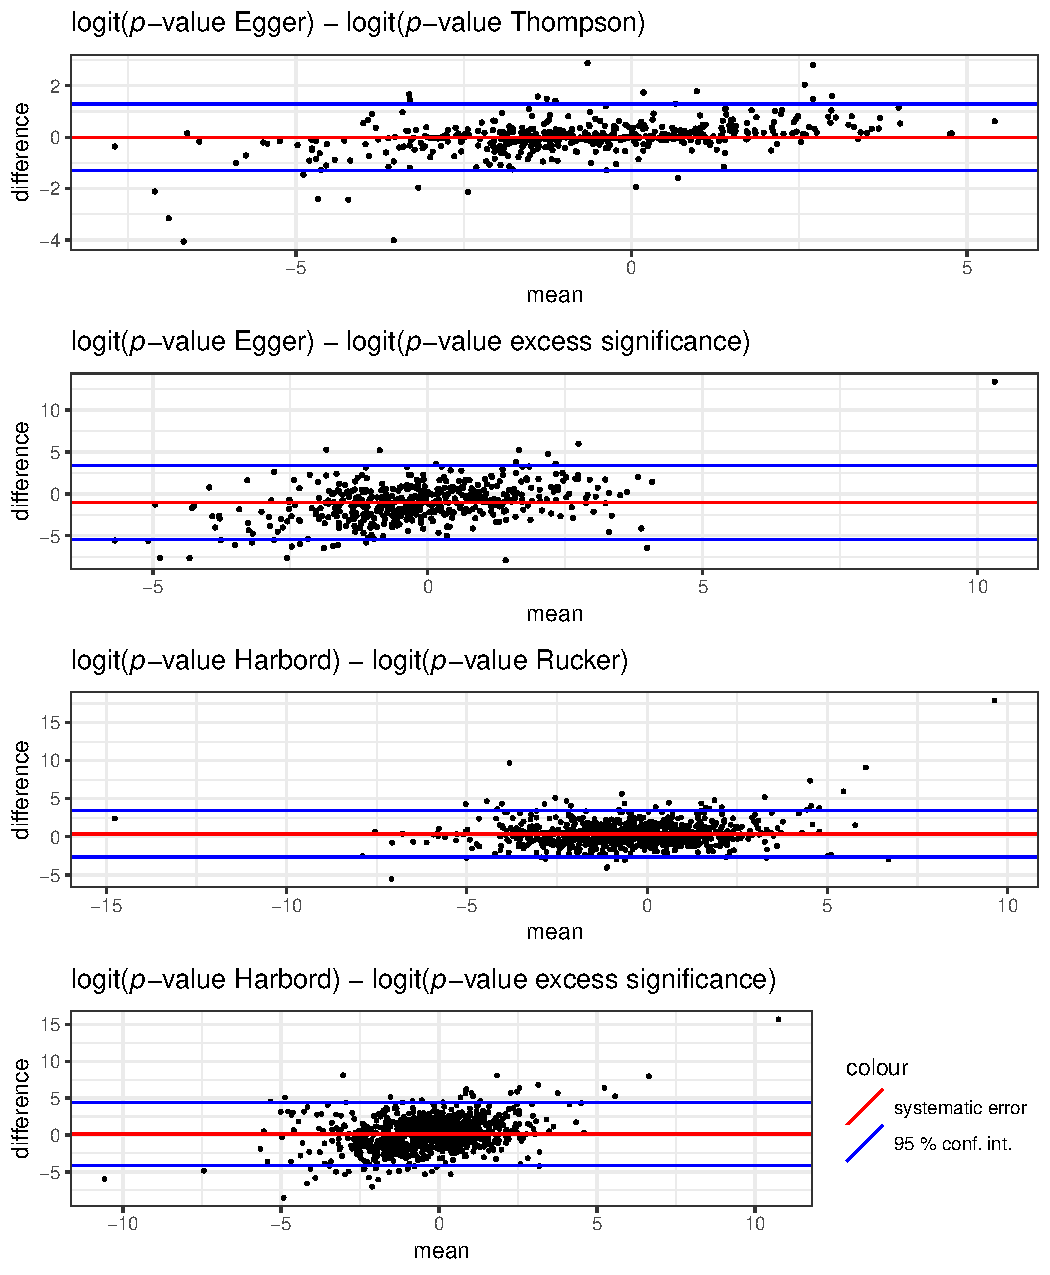
\includegraphics[width=\textwidth-3cm]{figure/ch02_figunnamed-chunk-13-1} 

}



\end{knitrout}
\caption{Overall fraction of studies whose treatment effect estimate was significant when pooled by means of meta-analysis. The fractions have been calculated
by fixed-effects, random-effects and Hartung and Knapp adjusted random-effects meta-analysis}
\label{primary.secondary.significance}
\end{figure}

What has been found is that even the meta-analysis that for all meta-analysis methods, the amount of secondary significance is higher than the amount of primary significance. Thus more primarily non-significant results can be attached to a secondarily significant result than vice-versa.

\vspace{0mm}
To illustrate this, the fraction of studies with significant primary treatment effect and primary non-significant treatment effect can be plotted separately (Figure \ref{primary.secondary.significance.sep.sig}). 

\begin{figure}
\begin{knitrout}
\definecolor{shadecolor}{rgb}{0.98, 0.98, 0.98}\color{fgcolor}

{\centering 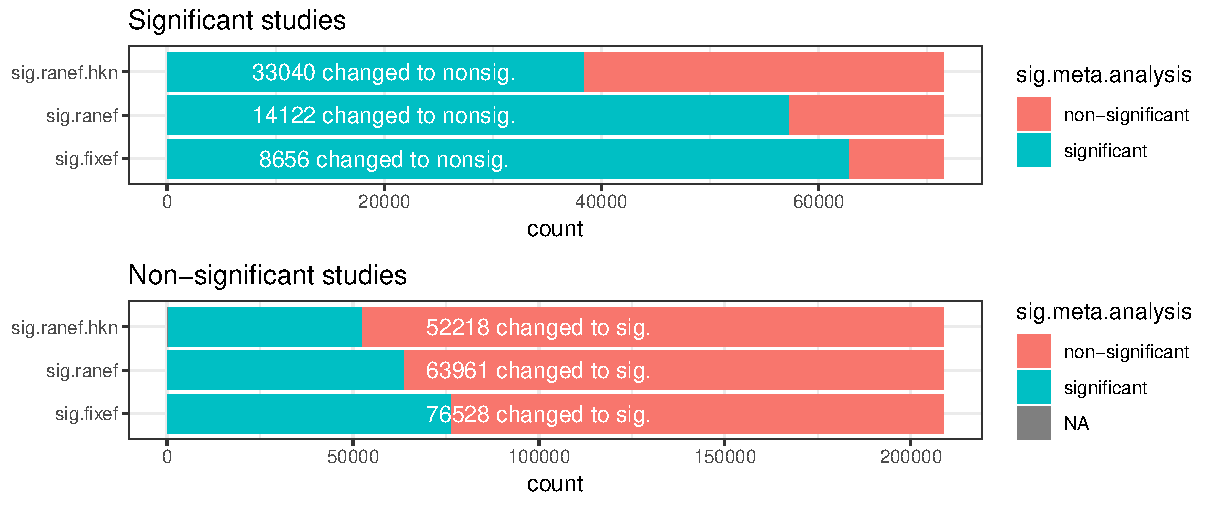
\includegraphics[width=\textwidth-3cm]{figure/ch02_figunnamed-chunk-14-1} 

}



\end{knitrout}
\caption{Overall fraction of studies whose treatment effect estimate was significant when pooled by means of meta-analysis, separated by significance of study treatment effect estimate. The fractions have been calculated
by fixed-effects, random-effects and Hartung and Knapp adjusted random-effects meta-analysis}
\label{primary.secondary.significance}
\end{figure}

It can be seen that the extent of overlap between primary and secondary significance varies between meta-analysis. A considerable amount of both primary significant and primary non-significant results are overruled by meta-analysis hypothesis tests. 


The amount of significant heterogeneity in the results used by the meta-analyses is 53350 and corresponds to 81.5936377\% of the total number of meta-analyses.

%Comparison of significance separated for significant Q? Chunck 2

%Proportion of significant pooled estimates based on proportion of single pooled estimates? Chunck 5


\section{Small study effects}



To provide an overview over the abundance of small study effects in the dataset, first it is shown how median absolute effect size decreases with increasing sample size of the results (Figure \ref{effect.samplesize}). 
%In some sense, this is the same idea as for a funnel plot, by depicting the size of effects relative to their variance. 

\vspace{0mm}
A clear trend of decrease of absolute effect size with increasing sample size (i.e. smaller variance) is visible. 
%It is particularly substantive from very small trials ($n$ = 10) to medium sample size ($n$ = 100) and afterwards it evens off. With increasing sample size, there are fewer results, therefore, the variation between medians increases. 
All effects are normalized by subtracting the mean effect size of the dataset and dividing through the standard deviation. Note that various types of outcome measures are included, such as mean difference and risk ratios, and are normalized with respect to all effects.

\begin{figure}
\begin{knitrout}
\definecolor{shadecolor}{rgb}{0.98, 0.98, 0.98}\color{fgcolor}

{\centering 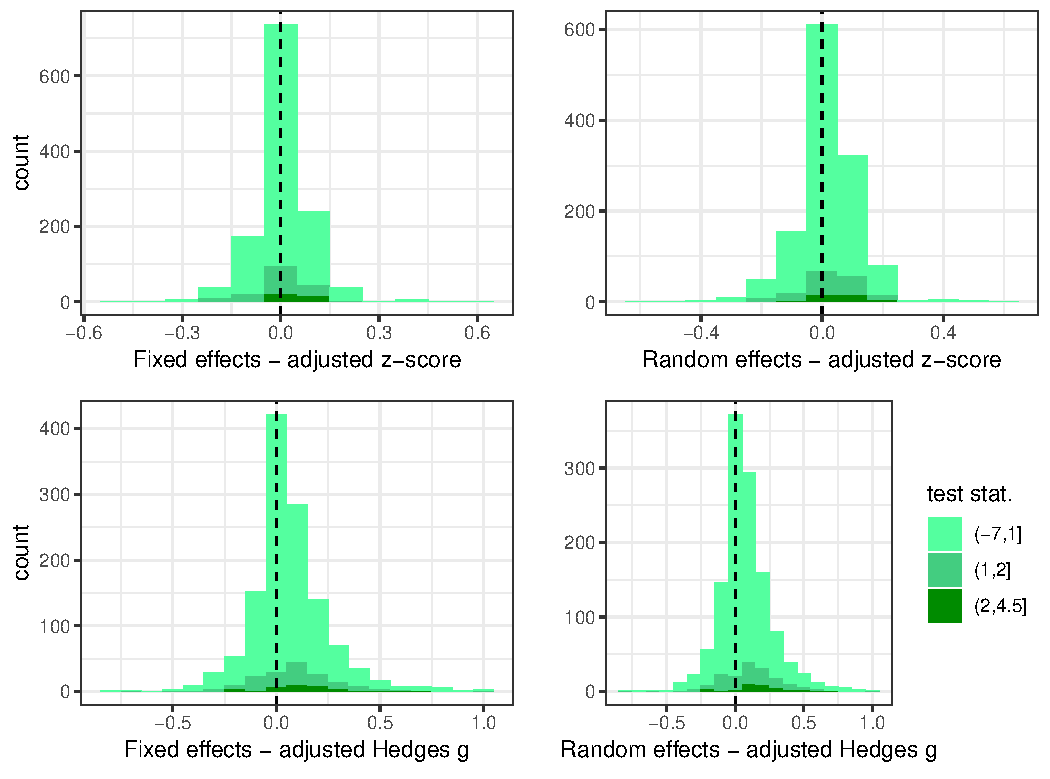
\includegraphics[width=\textwidth-3cm]{figure/ch02_figunnamed-chunk-16-1} 

}



\end{knitrout}
\caption{Median of the absolute value of the normalized effect size plotted against the total sample size.}
\label{effect.samplesize}
\end{figure}

The median absolute normalized effect size can be visualized for the different outcome measures separately (Figure \ref{effect.samplesize.separated}). The plot confirms the trend of median effect size decrease towards lower sample size (e.g. for Risk Ratios: decrease $> 0.1$ standard deviations from 10 to 50 study participants). Instead of normalizing the effects 
%(i.e. subtracting mean and dividing through the standard deviation) 
for all effect sizes, the effects are normalized with respect to the effects of the same outcome measures. 

\begin{figure}
\begin{knitrout}
\definecolor{shadecolor}{rgb}{0.98, 0.98, 0.98}\color{fgcolor}

{\centering 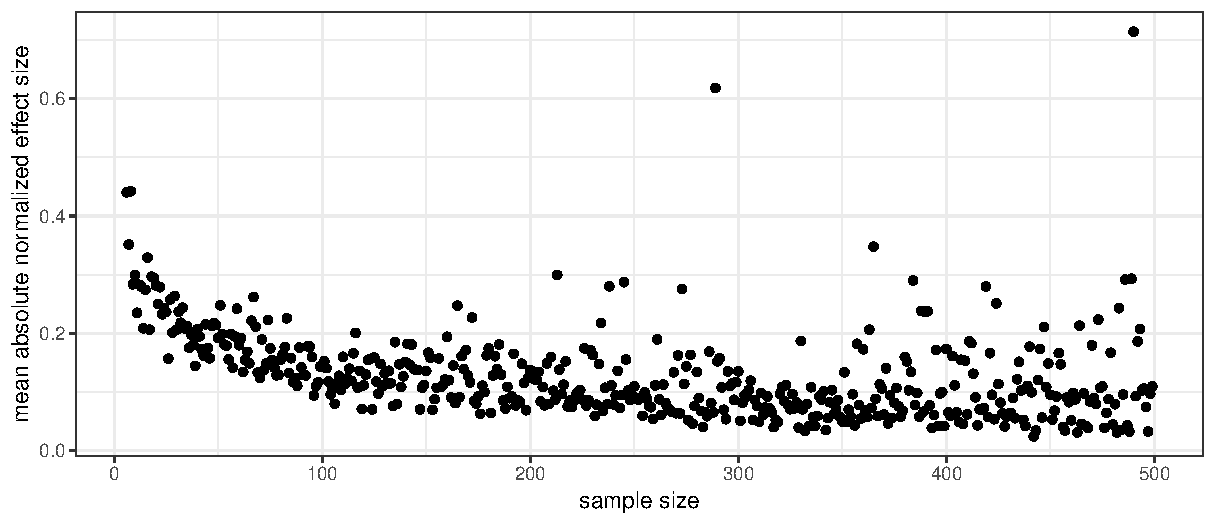
\includegraphics[width=\textwidth-3cm]{figure/ch02_figunnamed-chunk-17-1} 

}



\end{knitrout}
\caption{Median of the absolute value of the normalized effect size plotted against the total sample size, separated for outcome measures.}
\label{effect.samplesize.separated}
\end{figure}

%Show absolute effect size depending on scaled time? Chunck 3




\subsection{Small Study Effect Tests}



There are tests that can be applied to find out if small study effects are present in the meta analysis. For the precise description, see the methods section. Application of the tests is only recommended if there are ten or more studies \citep{cochrane.handbook} that can be used, so all meta-analyses with less than ten studies have been excluded.

\vspace{0mm}
There are modifications to make tests more appropriate in case of binary outcomes, therefore the results have been separated in continuous and dichotomous outcome test results. In Figure \ref{bias.results.cont} the proportion of test results that led to rejection of the null hypothesis of no small study effect based on the 5 \% level are shown for continuous outcomes ($n$ = 1383)
The same is shown in Figure \ref{bias.results.bin} for dichotomous outcome measures ($n$ = 3442). The amount of studies varies from 5\% (Schwarzer's Test) to 13 \% (Egger's Test) for binary outcomes and 9\% (Begg and Mazumdar's Test) to 25 \% (Egger's Test) for continuous outcomes. 


\begin{figure}
\begin{knitrout}
\definecolor{shadecolor}{rgb}{0.98, 0.98, 0.98}\color{fgcolor}

{\centering 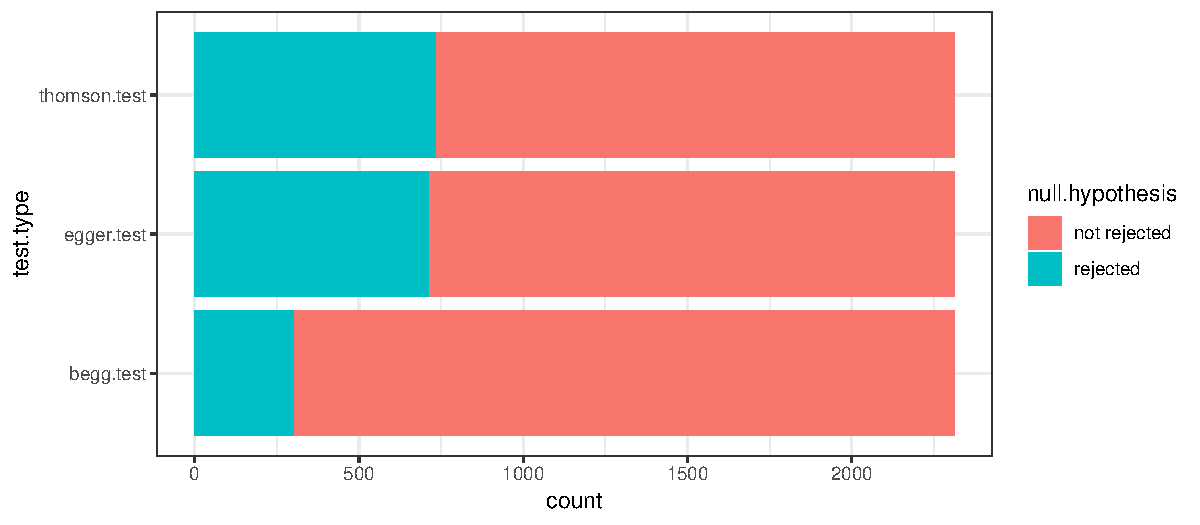
\includegraphics[width=\textwidth-3cm]{figure/ch02_figunnamed-chunk-19-1} 

}



\end{knitrout}
\caption{Proportion where the null hypothesis of no small study effect is rejected based on the 5\% significance level for different tests (continuous outcomes).}
\label{bias.results.cont}
\end{figure}

\begin{figure}
\begin{knitrout}
\definecolor{shadecolor}{rgb}{0.98, 0.98, 0.98}\color{fgcolor}

{\centering 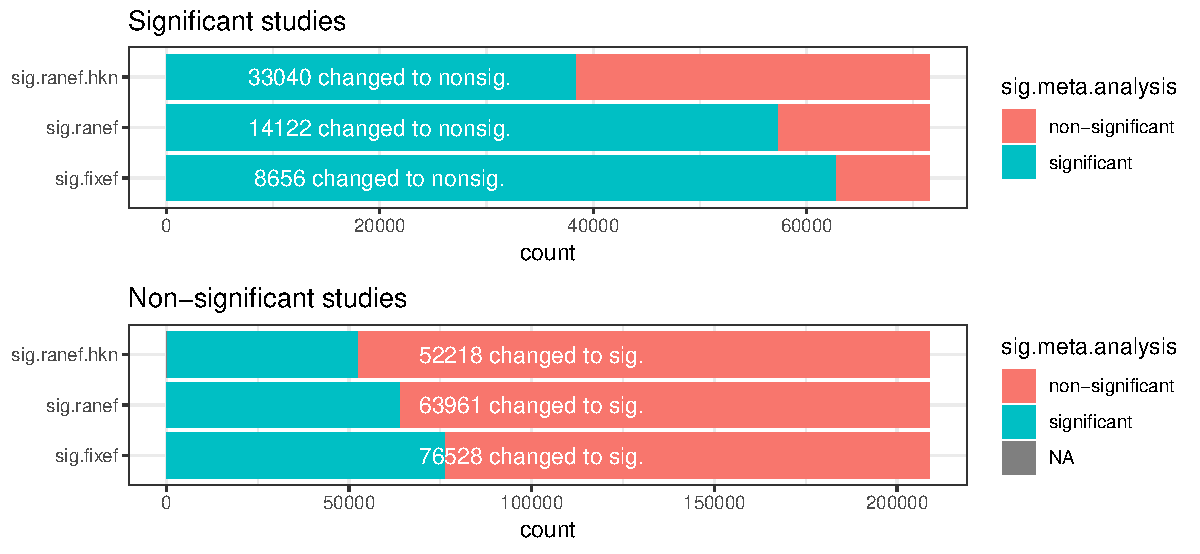
\includegraphics[width=\textwidth-3cm]{figure/ch02_figunnamed-chunk-20-1} 

}



\end{knitrout}
\caption{Proportion where the null hypothesis of no small study effect is rejected based on the 5\% significance level for different tests (dichotomous outcomes).}
\label{bias.results.bin}
\end{figure}

There is no substantive change in the fraction of positive test results, depending on if the pooled treatment effect size estimate is significant or not. Most substantively, the fraction of positive Egger Test results increases for significant pooled treatment effects by 0.0768414 (the minimal increase is 0.0103761 for Schwarzer's Test).

%Show plots of significant meta-analyses separated? Chunck 4

Furthermore one can look if the frequencies of tests that reject the null hypotheses change over time (mean publication year of the studies included in the meta analyses). The proportion of the test results are shown in Figure \ref{pub.bias.time.overtime}. The Figure suggests that the frequency of publication bias remains constant over time. The mean publication years have been restricted such that at least 180 meta-analyses are available per year, such that random fluctuation is restricted to some extent. The significance threshold for the $p$-values used is 0.05, and the small study effect test used is Thomson's test (with the arcsine variance stabilizing transformation function used in the case of binary outcomes).

\begin{figure}
\begin{knitrout}
\definecolor{shadecolor}{rgb}{0.98, 0.98, 0.98}\color{fgcolor}

{\centering 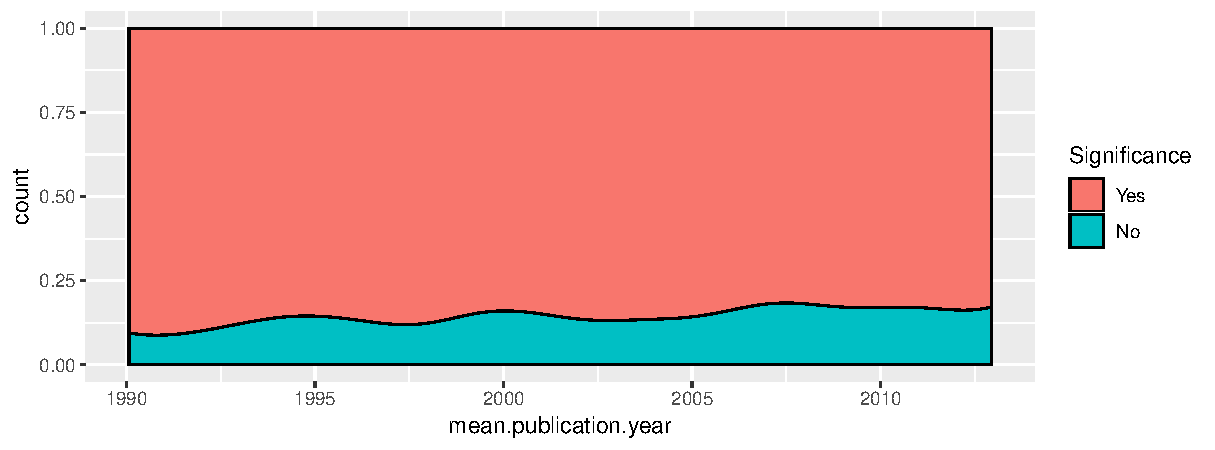
\includegraphics[width=\textwidth-3cm]{figure/ch02_figunnamed-chunk-21-1} 

}



\end{knitrout}
\caption{Proportion of test results where the null hypothesis of no small study effect is rejected over time (mean publication.year).}
\label{pub.bias.overtime}
\end{figure}


The agreement of the tests, i.e. the proportion of meta-analyses where the rest results are equal between tests, is shown in Table \ref{agreement.bin} and Table \ref{agreement.cont}, again separated for outcome types. Agreement in tests for binary outcomes is better than continuous outcomes, with some variation between tests (binary outcomes: 83 to 91\%). Correlation varies more between tests, both for continuous and binary outcome tests.

% latex table generated in R 3.5.1 by xtable 1.8-3 package
% Tue May  7 13:05:39 2019
\begin{table}[ht]
\centering
\begingroup\footnotesize
\begin{tabular}{lll}
  \hline
 & Test Agreement & P-value Correlation \\ 
  \hline
egger.schwarzer & 0.87 & 0.39 \\ 
  egger.peter & 0.89 & 0.51 \\ 
  egger.rucker & 0.88 & 0.48 \\ 
  egger.harbord & 0.93 & 0.76 \\ 
  schwarzer.peter & 0.89 & 0.29 \\ 
  schwarzer.rucker & 0.88 & 0.34 \\ 
  schwarzer.harbord & 0.92 & 0.51 \\ 
  rucker.peter & 0.92 & 0.67 \\ 
  harbord.peter & 0.91 & 0.52 \\ 
   \hline
\end{tabular}
\endgroup
\caption{Proportion of tests that agree in rejection ar acceptance of the null hypothesis that there is no small study effect (dichotomous outcomes)} 
\label{agreement.bin}
\end{table}



% latex table generated in R 3.5.1 by xtable 1.8-3 package
% Tue May  7 13:05:39 2019
\begin{table}[ht]
\centering
\begingroup\footnotesize
\begin{tabular}{lll}
  \hline
 & Test Agreement & P-value Correlation \\ 
  \hline
thomson.egger & 0.89 & 0.69 \\ 
  thomson.begg & 0.82 & 0.47 \\ 
  egger.begg & 0.79 & 0.36 \\ 
   \hline
\end{tabular}
\endgroup
\caption{Proportion of tests that agree in rejection ar acceptance of the null hypothesis that there is no small study effect (continuous outcomes)} 
\label{agreement.cont}
\end{table}


\vspace{0mm}
Test performance depends on the sample size, despite having restricted sample size to a minimum of 10 studies. The p-values of the Thompson and Sharp tests are shown with respect to the sample size of the meta-analysis in Figure \ref{pvalues.samplesize}. %(Suggests that 10 is likely too small)
In the case of binary outcomes, the arcsine variance stabilizing function has been applied prior to use of Thompson and Sharp's test. A trend towards more rejections for larger sample sizes can be seen.

\begin{figure}
\begin{knitrout}
\definecolor{shadecolor}{rgb}{0.98, 0.98, 0.98}\color{fgcolor}

{\centering 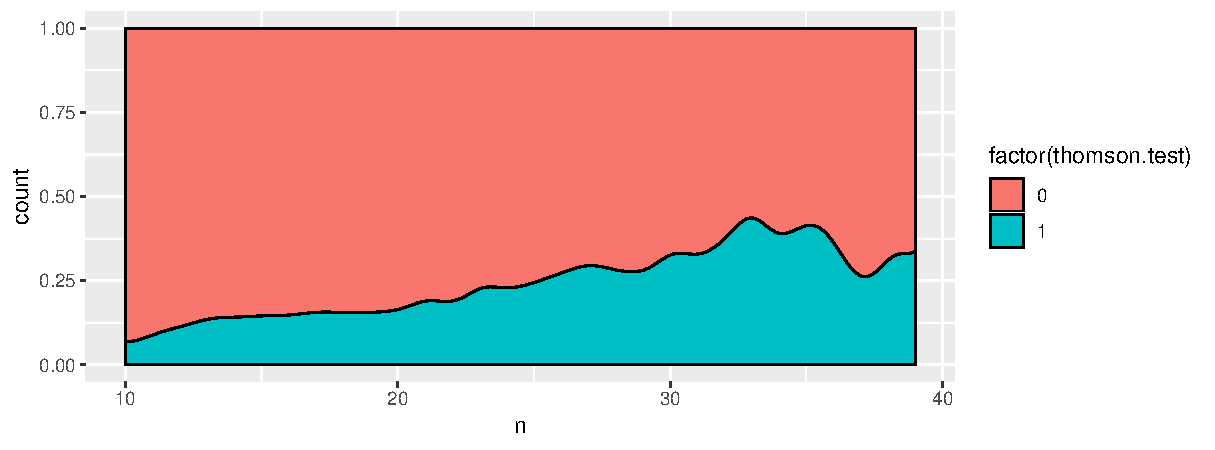
\includegraphics[width=\textwidth-3cm]{figure/ch02_figunnamed-chunk-24-1} 

}



\end{knitrout}
\caption{P-values of Thomson and Sharp's test for small study effects and their corresponding sample size.}
\label{pvalues.samplesize}
\end{figure}



\vspace{0mm}
One can use the proportion of added studies by the trim-and-fill method from the overall number of studies to further investigate the extent of small study effects. The mean fraction of trimmed comparisons for binary outcomes is 0.19 and the median 0.18. 
% A histogram with those fractions is shown in Figure \ref{trimfill.cont} for continuous outcomes and \ref{trimfill.bin} for dichotomous outcomes. In both cases, the method very commonly adds supposedly unpublished studies to the meta-analyses. 
In Figure \ref{trimfill.pvalues.bin} and Figure \ref{trimfill.pvalues.cont}, the relationship between fraction of added studies by trim-and-fill and the hypothesis test decisions of the small study effects tests is shown for continuous and dichotomous outcomes. In the case of Peters test dor dichotomous outcomes, there is less agreement with the trim-and fill method than in the case of Thomson and Sharp's test for continuos outcomes in the sense that the fraction of meta-analyses with rejected null hypothesises increases more clearly when there are more studies added by trim-and-fill. 

\begin{figure}
\begin{knitrout}
\definecolor{shadecolor}{rgb}{0.98, 0.98, 0.98}\color{fgcolor}

{\centering 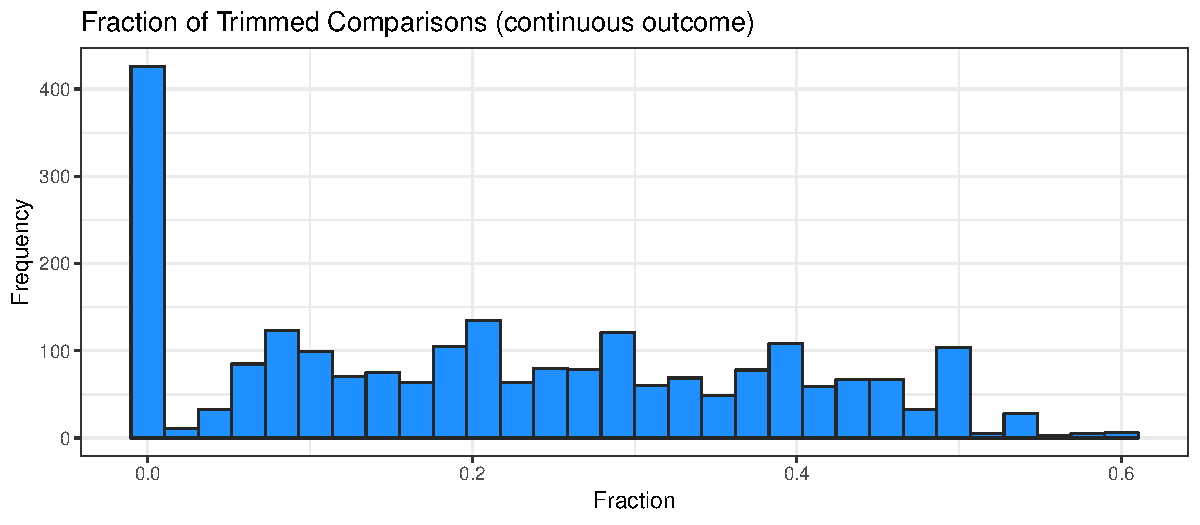
\includegraphics[width=\textwidth-3cm]{figure/ch02_figunnamed-chunk-25-1} 

}



\end{knitrout}
\caption{Fraction of added studies for small study effect correction by trim and fill and the corresponding small study effect test decision (based on 5\% significance level) of Peters test and dichotomous outcomes}
\label{trimfill.pvalues.bin}
\end{figure}

\begin{figure}
\begin{knitrout}
\definecolor{shadecolor}{rgb}{0.98, 0.98, 0.98}\color{fgcolor}

{\centering 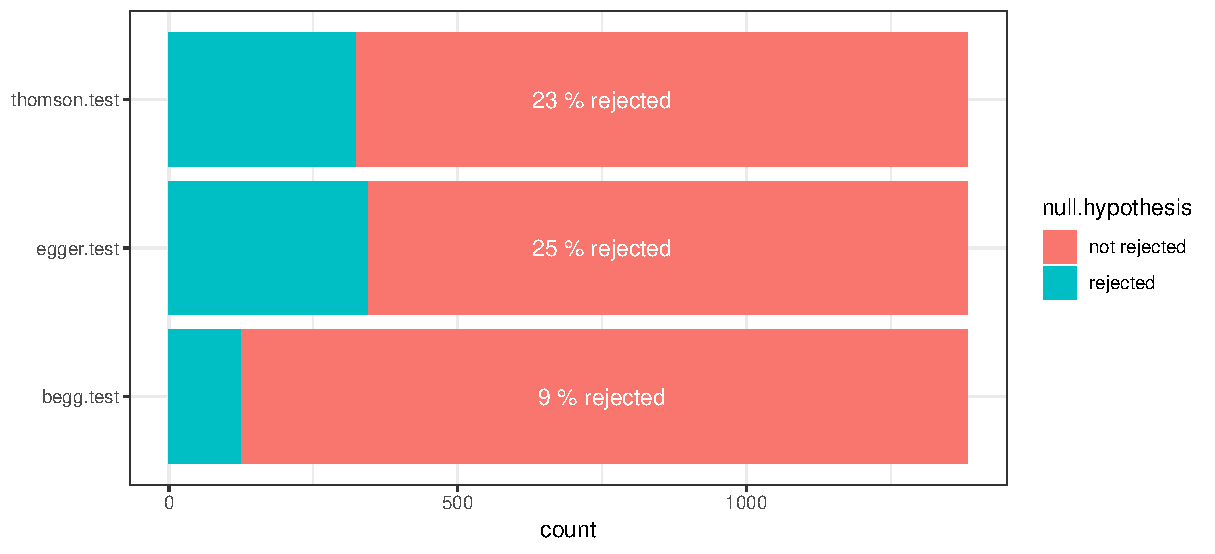
\includegraphics[width=\textwidth-3cm]{figure/ch02_figunnamed-chunk-26-1} 

}



\end{knitrout}
\caption{Fraction of added studies for small study effect correction by trim and fill and the corresponding small study effect test decision (based on 5\% significance level) of Thomson and Sharp's test and continuous outcomes}
\label{trimfill.pvalues.cont}
\end{figure}


\subsection{Small Study Effect Correction}
Multiple methods are available to correct for the effects of small study effects in order to get an unbiased estimate. Three of them will be applied to the meta-analyses shown previously that have ten or more study results and are therefore eligible for testing for publication bias. 

\vspace{0mm}
The extent to what the results of the meta-analysis results are changed can be investigated. Because statistical significance is often used to decide if there is a treatment effect, a non-significant corrected effect size estimate can indicate that an observed treatment effect has been accepted because of small study effects. Therefore, the cases have been counted in which 
\begin{enumerate}
\item Significance or non-significance of pooled estimate of meta-analysis did not change after correction for small study effects.
\item Significance of pooled estimate of meta-analysis did change to non-significance after correction for small study effects.
\item Non-significance of pooled estimate of meta-analysis did change to significance after correction for small study effects.
\end{enumerate}

The results of this can be seen in Figure \ref{significance.change.fixed} for all three methods, comparing the significance of the corrected pooled effect size estimate with the significance of the pooled effect size estimate of the fixed effects meta-analysis. The same for significance of random effects meta-analysis is shown in Figure \ref{significance.change.random}. The significance threshold was chosen such that the $p$-value had to be < 0.05 for rejection of the null hypothesis of no treatment effect. The correction methods were trim-and-fill, copas selection model and regression with random effects and shrinkage of within-study-variance methods. More details to the applied correction methods and their application are in the methods section \ref{methods}. Notably, the correction methods has been applied to all meta-analyses, thus also for such that had no significant small study effect test result. 


\begin{figure}
\begin{knitrout}
\definecolor{shadecolor}{rgb}{0.98, 0.98, 0.98}\color{fgcolor}

{\centering 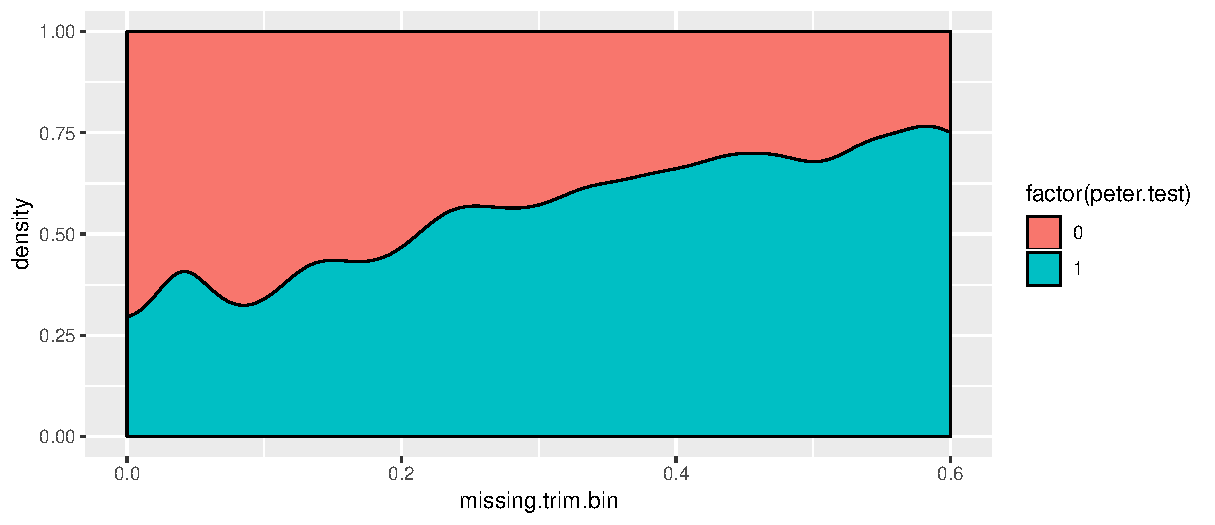
\includegraphics[width=\textwidth-3cm]{figure/ch02_figunnamed-chunk-27-1} 

}



\end{knitrout}
\caption{Change in signficance of fixed effects meta-analysis pooled estimate after correction.}
\label{significance.change.fixed}
\end{figure}

\begin{figure}
\begin{knitrout}
\definecolor{shadecolor}{rgb}{0.98, 0.98, 0.98}\color{fgcolor}

{\centering 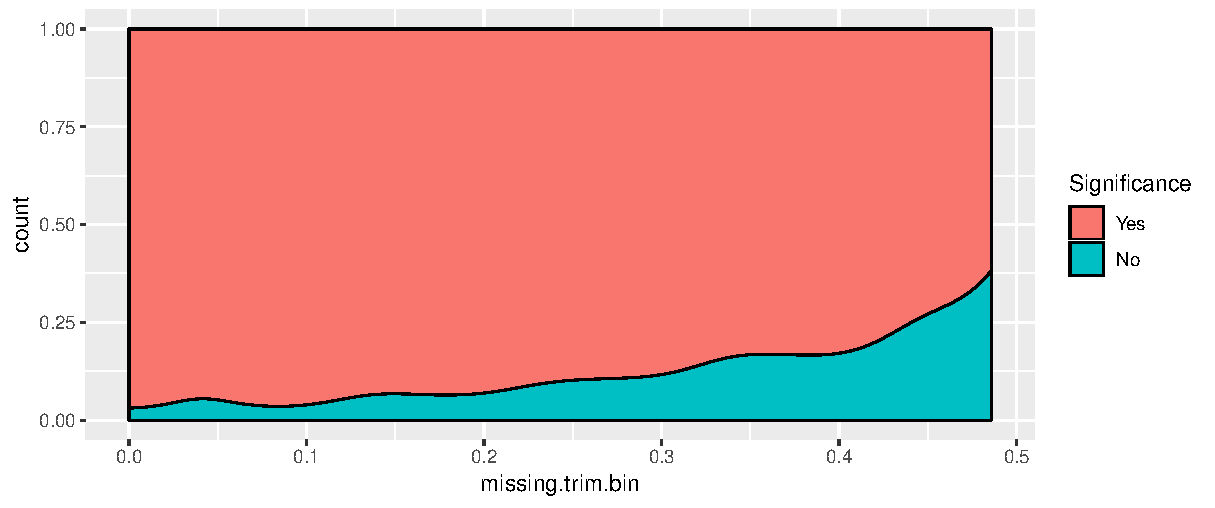
\includegraphics[width=\textwidth-3cm]{figure/ch02_figunnamed-chunk-28-1} 

}



\end{knitrout}
\caption{Change in signficance of random effects meta-analysis pooled estimate after correction.}
\label{significance.change.random}
\end{figure}

Since it has been previously seen in Figure \ref{test.results} that the results of small study effects vary considerably between continuous outcomes, the results in significance change from fixed effects meta-analysis can be seen separately in Figure \ref{significance.change.fixed.sep} for continuous and binary outcomes. The change in significance from random effects meta-analysis to significance of corrected estimate can be seen in Figure \ref{significance.change.fixed.sep}

\begin{figure}
\begin{knitrout}
\definecolor{shadecolor}{rgb}{0.98, 0.98, 0.98}\color{fgcolor}

{\centering 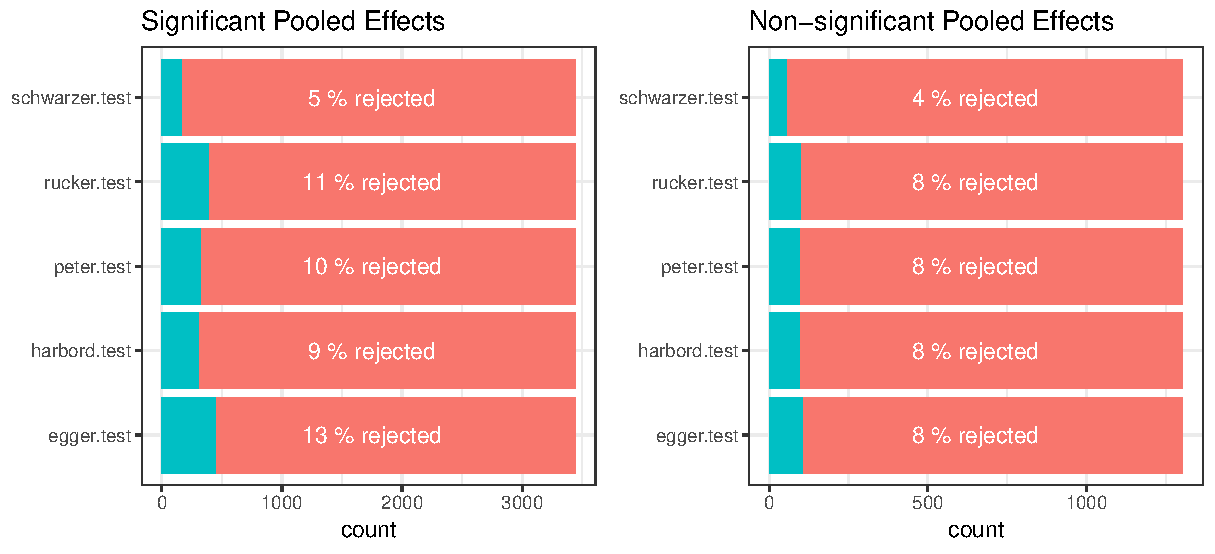
\includegraphics[width=\textwidth-3cm]{figure/ch02_figunnamed-chunk-29-1} 

}



\end{knitrout}
\caption{Change in signficance of fixed effects meta-analysis pooled estimate after correction, separated for continuous and binary outcomes.}
\label{significance.change.fixed.sep}
\end{figure}

\begin{figure}
\begin{knitrout}
\definecolor{shadecolor}{rgb}{0.98, 0.98, 0.98}\color{fgcolor}

{\centering 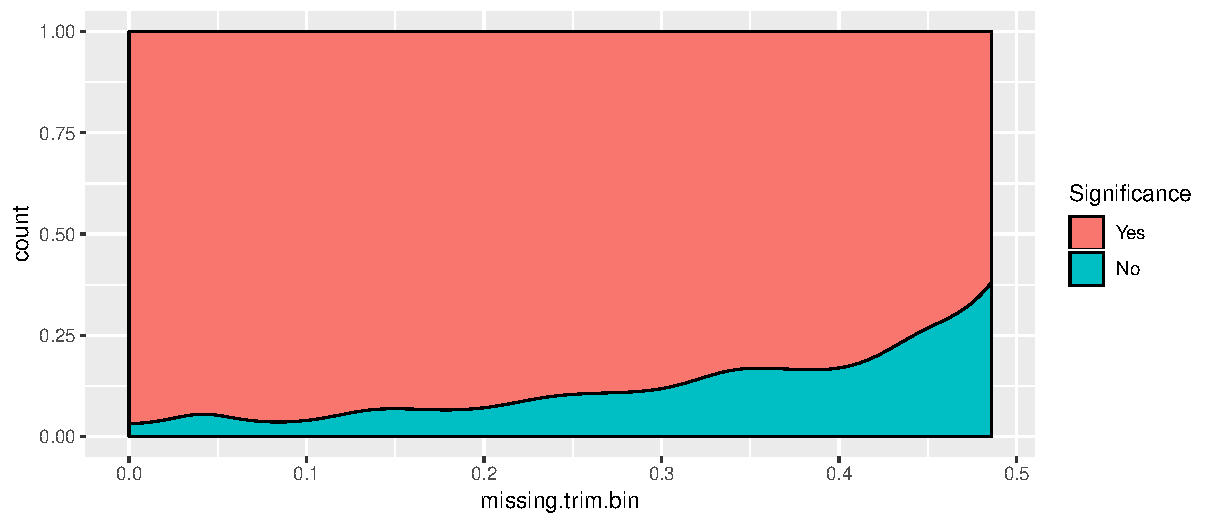
\includegraphics[width=\textwidth-3cm]{figure/ch02_figunnamed-chunk-30-1} 

}



\end{knitrout}
\caption{Change in signficance of random effects meta-analysis pooled estimate after correction, separated for continuous and binary outcomes.}
\label{significance.change.random}
\end{figure}

Because the real amount of publication bias in the dataset is not known, the correction method can also be applied only to meta-analyses that have publication bias according to the small study effect tests in the previous section. Because the test developed by \citet{thomson.sharp} has been applied to both binary and continuous outcome meta-analyses (in the case of binary outcomes to arcsine variance stabilized proportions), it is used as a criterium to distinguish biased from unbiased meta-analyses. The proportions of significance tests of pooled treatment effects that turned from significant to non-significant, non-significant to significant etc. are shown in Figure \ref{significance.change.fixed.sep}. Fixed effects meta-analysis has been used to determine signficance of the uncorrected estimate.


\begin{figure}
\begin{knitrout}
\definecolor{shadecolor}{rgb}{0.98, 0.98, 0.98}\color{fgcolor}

{\centering 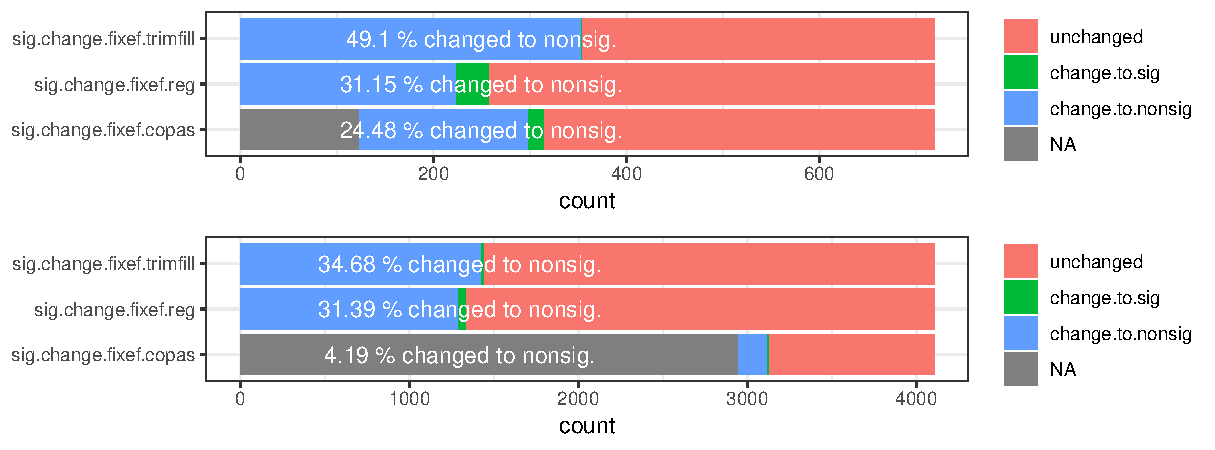
\includegraphics[width=\textwidth-3cm]{figure/ch02_figunnamed-chunk-31-1} 

}



\end{knitrout}
\caption{Change in signficance of random effects meta-analysis pooled estimate after correction, separated for continuous and binary outcomes.}
\label{significance.change.random}
\end{figure}

Similarly, the number of missing studies per meta-analysis, i.e. those which have not been included because of small study effects, are estimated by the copas and trim-and-fill method and their empirical distribution is shown in histograms in Figure \ref{missing.studies.distribution}. For visualisation, the fraction of unpublished studies from the total fraction of available studies is shown.

\begin{figure}
\begin{knitrout}
\definecolor{shadecolor}{rgb}{0.98, 0.98, 0.98}\color{fgcolor}

{\centering 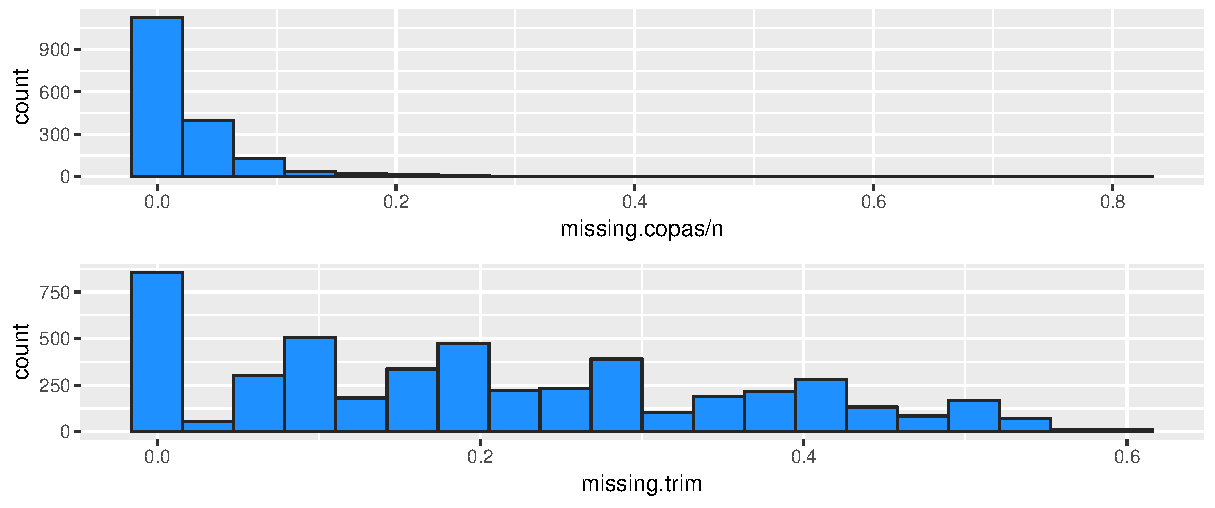
\includegraphics[width=\textwidth-3cm]{figure/ch02_figunnamed-chunk-32-1} 

}



\end{knitrout}
\caption{Fraction of missing studies estimated of the number of total studies included in the meta-analysis for copas selection and trim-and-fill method.}
\label{missing.studies.distribution}
\end{figure}




% # <<results = 'asis', Echo = FALSE>>=
% # rejection.bin <- meta.bin %>% summarize(egger.rejection = mean(egger.test),
% #                                             schwarzer.rejection = mean(schwarzer.test),
% #                                             rucker.rejection = mean(rucker.test),
% #                                             harbord.rejection = mean(harbord.test),
% #                                             peter.rejection = mean(peter.test))
% # print(xtable(rejection.bin), label = "bias.results", caption = "Cumulative number of groups with number of reproduction trials >= n", align = "llll", digits = 0), include.rownames = F, size = "footnotesize")
% # @






% 
% For continuous outcomes, three tests are available: Eggers (based on linear regression), Thompson and Sharp (weighted linear regression) and Begg and Mazumdar (rank based) test. The following three figures show the distribution of p-values of the corresponding tests. Note that only meta analyses with more than 10 comparisons have been included. 
% 
% \vspace{0mm}
% Since each histogram of p-values has 20 bins, the content of the bin with the smallest p-values is equal to the number of meta-analyses whose reporting bias test reports a p-value < 0.05. The fraction of those analyses in which we would reject the null-hypothesis based on the 5 \% threshold can therefore be assessed by eye, and would be for example for Eggers test somewhat less than one third of all analyses. 
% 
% \begin{figure}
% <<echo=FALSE>>=
% data %>% filter(outcome.measure == "Mean Difference" | outcome.measure == "Std. Mean Difference") %>% #filter(file.nr < 503) %>% 
%   filter(sd1 > 0 & sd2 > 0 ) %>% filter(!is.na(sd1) & !is.na(sd2)) %>% 
%   filter(mean1 != 0 | mean2 != 0 ) %>% filter(!is.na(mean1) & !is.na(mean2)) %>% 
%   group_by(file.nr, outcome.nr, subgroup.nr) %>% 
%   mutate(n = n()) %>% filter(n > 9) %>% 
%   summarize(pval = metabias(metacont(n.e = total1, mean.e = mean1, sd.e = sd1, n.c = total2, mean.c = mean2, sd.c = sd2), 
%                             method = "linreg")$p.val) %>% 
%   ggplot(aes(x = pval)) + geom_histogram(col = "gray15", fill = "dodgerblue", bins = 20) +
%   theme_bw() + labs(title = "Eggers Reporting Bias Test P-values for Continuous Outcome Meta-Analyses") + xlab("P-value") + ylab("Frequency")
% @
% \caption{Histogram of p-values for Eggers reporting bias test (linear regression based) for continuous outcome meta analysis.}
% \label{egger.cont}
% \end{figure}
% 
% 
% \begin{figure}
% <<echo=FALSE>>=
% data %>% filter(outcome.measure == "Mean Difference" | outcome.measure == "Std. Mean Difference") %>% #filter(file.nr < 503) %>% 
%   filter(sd1 > 0 & sd2 > 0 ) %>% filter(!is.na(sd1) & !is.na(sd2)) %>% 
%   filter(mean1 != 0 | mean2 != 0 ) %>% filter(!is.na(mean1) & !is.na(mean2)) %>% 
%   group_by(file.nr, outcome.nr, subgroup.nr) %>% 
%   mutate(n = n()) %>% filter(n > 9) %>% 
%   summarize(pval = metabias(metacont(n.e = total1, mean.e = mean1, sd.e = sd1, n.c = total2, mean.c = mean2, sd.c = sd2), 
%                             method = "mm")$p.val) %>% 
%   ggplot(aes(x = pval)) + geom_histogram(col = "gray15", fill = "dodgerblue", bins = 20) +
%   theme_bw() + labs(title = "Thomson Sharp Reporting Bias Test P-values for Continuous Outcome Meta-Analyses") + xlab("P-value") + ylab("Frequency")
% @
% \caption{Histogram of p-values for Thompsom and Sharp reporting bias test (weighted linear regression based) for continuous outcome meta analysis.}
% \label{thomson.cont}
% \end{figure}
% 
% \begin{figure}
% <<echo=FALSE>>=
% data %>% filter(outcome.measure == "Mean Difference" | outcome.measure == "Std. Mean Difference") %>% #filter(file.nr < 503) %>% 
%   filter(sd1 > 0 & sd2 > 0 ) %>% filter(!is.na(sd1) & !is.na(sd2)) %>% 
%   filter(mean1 != 0 | mean2 != 0 ) %>% filter(!is.na(mean1) & !is.na(mean2)) %>% 
%   group_by(file.nr, outcome.nr, subgroup.nr) %>% 
%   mutate(n = n()) %>% filter(n > 9) %>% 
%   summarize(pval = metabias(metacont(n.e = total1, mean.e = mean1, sd.e = sd1, n.c = total2, mean.c = mean2, sd.c = sd2), 
%                             method = "rank")$p.val) %>% 
%   ggplot(aes(x = pval)) + geom_histogram(col = "gray15", fill = "dodgerblue", bins = 20) +
%   theme_bw() + labs(title = "Begg and Mazumdar Reporting Bias Test P-values for Continuous Outcome Meta-Analyses") + xlab("P-value") + ylab("Frequency")
% @
% \caption{Histogram of p-values for Begg and Mazumdar reporting bias test (rank based) for continuous outcome meta analysis.}
% \label{begg.cont}
% \end{figure}
% 
% 
% For binary outcomes, Peters and Harbords reporting bias test have been chosen. Also here, only meta-analyses with more than 10 comparisons are included.
% 
% \begin{figure}
% <<echo=FALSE>>=
% data %>% filter(outcome.measure == "Risk Ratio" | outcome.measure == "Odds Ratio") %>% filter(file.nr != 3014) %>% 
%   filter(events1 > 0 | events2 > 0) %>% 
%   filter(total1 - events1 > 0 | total2 - events2 > 0) %>%
%   group_by(file.nr, outcome.nr, subgroup.nr) %>% 
%   mutate(n = n()) %>% filter(n > 9) %>% 
%   summarize(pval = metabias(metabin(event.e = events1, n.e = total1, event.c = events2, n.c = total2, sm = "OR"), method = "peters")$p.val) %>% 
%   ggplot(aes(x = pval)) + geom_histogram(col = "gray15", fill = "dodgerblue", bins = 20) +
%   theme_bw() + labs(title = "Peters Reporting Bias Test P-values for Binary Outcome Meta-Analyses") + xlab("P-value") + ylab("Frequency")
% @
% \caption{Histogram of p-values for Peters reporting bias test (rank based) for continuous outcome meta analysis.}
% \label{peters.bin}
% \end{figure}
% 
% 
% \begin{figure}
% <<echo=FALSE>>=
% data %>% filter(outcome.measure == "Risk Ratio" | outcome.measure == "Odds Ratio") %>% filter(file.nr != 3014) %>% 
%   filter(events1 > 0 | events2 > 0) %>% 
%   filter(total1 - events1 > 0 | total2 - events2 > 0) %>%
%   group_by(file.nr, outcome.nr, subgroup.nr) %>% 
%   mutate(n = n()) %>% filter(n > 9) %>% 
%   summarize(pval = metabias(metabin(event.e = events1, n.e = total1, event.c = events2, n.c = total2, sm = "OR"), method = "score")$p.val) %>% 
%   ggplot(aes(x = pval)) + geom_histogram(col = "gray15", fill = "dodgerblue", bins = 20) +
%   theme_bw() + labs(title = "Harbord Reporting Bias Test P-values for Binary Outcome Meta-Analyses") + xlab("P-value") + ylab("Frequency")
% @
% \caption{Histogram of p-values for Harbord reporting bias test (rank based) for continuous outcome meta analysis.}
% \label{harbord.bin}
% \end{figure}


%%%%%%%%%%%%%%%%%%%%%%%%%%%%%%%%%%%%%%%%%%%%%%%%%%%%%%%%%%%%%%%%%%%%%%%%%%%%%%%%%%%%%%%%%%%%%%%%%%%%%%%%%%%%%%%%%%%%%%%%
%Chunck 1
%%%%%%%%%%%%%%%%%%%%%%%%%%%%%%%%%%%%%%%%%%%%%%%%%%%%%%%%%%%%%%%%%%%%%%%%%%%%%%%%%%%%%%%%%%%%%%%%%%%%%%%%%%%%%%%%%%%%%%%%
%%%%%%%%%%%%%%%%%%%%%%%%%%%%%%%%%%%%%%%%%%%%%%%%%%%%%%%%%%%%%%%%%%%%%%%%%%%%%%%%%%%%%%%%%%%%%%%%%%%%%%%%%%%%%%%%%%%%%%%%

% Since most of the times the study publication year is available for a given result, the fraction of significant treatment effects found is shown over time in Figure \ref{study.significance.overtime}. The $p$-value was chosen to be 0.05  only times where a reasonbly large number of effect estimates is available is shown in order to reduce random fluctuation ($n$ > 800). 
% 
% \begin{figure}
% <<echo=FALSE, warning=FALSE>>=
% data.ext %>% filter(!is.na(sig.type)) %>%  ggplot(aes(x = study.year, fill = factor(sig.type), stat(count))) + geom_density(na.rm = T, position = "fill") + 
%   labs(fill = "Significance") + scale_fill_discrete(labels= c("Yes", "No"))+ scale_x_continuous(limits = c(1970, 2017))
% @
% \caption{Mean of the absolute value of the normalized effect size plotted against the total sample size.}
% \label{study.significance.overtime}
% \end{figure}

%%%%%%%%%%%%%%%%%%%%%%%%%%%%%%%%%%%%%%%%%%%%%%%%%%%%%%%%%%%%%%%%%%%%%%%%%%%%%%%%%%%%%%%%%%%%%%%%%%%%%%%%%%%%%%%%%%%%%%%%
%Chunck 2
%%%%%%%%%%%%%%%%%%%%%%%%%%%%%%%%%%%%%%%%%%%%%%%%%%%%%%%%%%%%%%%%%%%%%%%%%%%%%%%%%%%%%%%%%%%%%%%%%%%%%%%%%%%%%%%%%%%%%%%%
%%%%%%%%%%%%%%%%%%%%%%%%%%%%%%%%%%%%%%%%%%%%%%%%%%%%%%%%%%%%%%%%%%%%%%%%%%%%%%%%%%%%%%%%%%%%%%%%%%%%%%%%%%%%%%%%%%%%%%%%

% The separation of studies can also be made based on the significance of heterogeneity between them when pooling them by means of a meta-analysis. Significant heterogeneity between studies corresponds to a rejection of the null-hypothesis that all the study treatment effect estimates share the same underlying distribution. The test used to assess heterogeneity was based on the between-study heterogeneity estimate $Q$ estimated as \citet{tau.estimator} suggested. This is shown in Figure \ref{primary.secondary.significance.sep.sig}.
% 
% \begin{figure}
% <<echo=FALSE, warning=FALSE>>=
% grid.arrange(sig.meta.Q1, nonsig.meta.Q, ncol= 1)
% @
% \caption{Overall fraction of studies whose treatment effect estimate was significant when pooled by means of meta-analysis, separated by significance of study treatment effect estimate. The fractions have been calculated
% by fixed-effects, random-effects and Hartung and Knapp adjusted random-effects meta-analysis}
% \label{primary.secondary.significance.sep.sig}
% \end{figure}

%%%%%%%%%%%%%%%%%%%%%%%%%%%%%%%%%%%%%%%%%%%%%%%%%%%%%%%%%%%%%%%%%%%%%%%%%%%%%%%%%%%%%%%%%%%%%%%%%%%%%%%%%%%%%%%%%%%%%%%%
%Chunck 3
%%%%%%%%%%%%%%%%%%%%%%%%%%%%%%%%%%%%%%%%%%%%%%%%%%%%%%%%%%%%%%%%%%%%%%%%%%%%%%%%%%%%%%%%%%%%%%%%%%%%%%%%%%%%%%%%%%%%%%%%
%%%%%%%%%%%%%%%%%%%%%%%%%%%%%%%%%%%%%%%%%%%%%%%%%%%%%%%%%%%%%%%%%%%%%%%%%%%%%%%%%%%%%%%%%%%%%%%%%%%%%%%%%%%%%%%%%%%%%%%%

% A second way to analyse meta-analyses is a cumulative meta-analysis that should reveal shifts in treatment effect sizes over time. This can again be done for the entire dataset, i.e. for all effect estimates and their ordering in time. It is important to scale the effect estimates here with respect to the estimates of the replication studies that are about the same subject, have the same outcome measure, etc. Also, only effect estimates that can be compared to other estimates before are included, i.e. only study results with one or more replica are included. Time needs to be scaled and normalized in order to compare multiple time-trends in effect size to each other and gain insights in the overall trend. This is done in Figure \ref{effects.overtime.separated}, separared for odds rati, risk ratio, and mean and standardized difference outcome measures. In order to reduce the spread over time of effect sizes, only studies between 1970 and 2019 were included, as well as studies with a minimal group size of 12 participants (each group).
% 
% \begin{figure}
% <<echo=FALSE>>=
% data.ext %>% filter(outcome.measure.new == "Mean Difference" | outcome.measure.new == "Std. Mean Difference" | 
%                 outcome.measure.new == "Risk Ratio" | outcome.measure.new == "Odds Ratio") %>% 
%   filter(total1 > 11 & total2 > 11) %>% filter(!is.na(study.year) & study.year > 1970 & study.year < 2019) %>% 
%   group_by(meta.id) %>% mutate(n = n()) %>% filter(n > 1) %>% 
%   mutate(scaled.effect = abs(scale(effect)), scaled.time = scale(study.year)) %>% 
%   ggplot(aes(x = scaled.time, y = scaled.effect)) + geom_point(size = .5, alpha = 0.2)  + facet_wrap(~outcome.measure.new) +
%   geom_smooth() + theme_bw() +  ylab("absolute scaled effect")  + ylab("scaled time")
% @
% \caption{Absolute values of scaled effect sizes over scaled time, separated for outcome measures.}
% \label{effects.overtime.separated}
% \end{figure}

%%%%%%%%%%%%%%%%%%%%%%%%%%%%%%%%%%%%%%%%%%%%%%%%%%%%%%%%%%%%%%%%%%%%%%%%%%%%%%%%%%%%%%%%%%%%%%%%%%%%%%%%%%%%%%%%%%%%%%%%
%Chunck 4
%%%%%%%%%%%%%%%%%%%%%%%%%%%%%%%%%%%%%%%%%%%%%%%%%%%%%%%%%%%%%%%%%%%%%%%%%%%%%%%%%%%%%%%%%%%%%%%%%%%%%%%%%%%%%%%%%%%%%%%%
%%%%%%%%%%%%%%%%%%%%%%%%%%%%%%%%%%%%%%%%%%%%%%%%%%%%%%%%%%%%%%%%%%%%%%%%%%%%%%%%%%%%%%%%%%%%%%%%%%%%%%%%%%%%%%%%%%%%%%%%

% The same plots can be shown separately for meta-analyses with significant and non-significant pooled effect sizes. This is done in Figure \ref{bias.results.cont.sep} for continuous outcomes and \ref{bias.results.bin.sep} for binary outcomes.
% 
% \begin{figure}
% <<echo=FALSE, warning=FALSE>>=
% grid.arrange(p3, p4, ncol = 2)
% @
% \caption{Proportion where the null hypothesis of no small study effect is rejected based on the 5\% significance level for different tests (continuous outcomes).}
% \label{bias.results.cont.sep}
% \end{figure}
% 
% \begin{figure}
% <<echo=FALSE, warning=FALSE>>=
% grid.arrange(p1, p2, ncol = 2)
% @
% \caption{Proportion where the null hypothesis of no small study effect is rejected based on the 5\% significance level for different tests (dichotomous outcomes).}
% \label{bias.results.bin.sep}
% \end{figure}

%%%%%%%%%%%%%%%%%%%%%%%%%%%%%%%%%%%%%%%%%%%%%%%%%%%%%%%%%%%%%%%%%%%%%%%%%%%%%%%%%%%%%%%%%%%%%%%%%%%%%%%%%%%%%%%%%%%%%%%%
%Chunck 5
%%%%%%%%%%%%%%%%%%%%%%%%%%%%%%%%%%%%%%%%%%%%%%%%%%%%%%%%%%%%%%%%%%%%%%%%%%%%%%%%%%%%%%%%%%%%%%%%%%%%%%%%%%%%%%%%%%%%%%%%
%%%%%%%%%%%%%%%%%%%%%%%%%%%%%%%%%%%%%%%%%%%%%%%%%%%%%%%%%%%%%%%%%%%%%%%%%%%%%%%%%%%%%%%%%%%%%%%%%%%%%%%%%%%%%%%%%%%%%%%%

% #Proportion of significant pooled estimates based on proportion of single pooled estimates
% mly %>% filter(NA.sig.type == 0) %>% ggplot(aes(x = mean.sig.type)) + geom_histogram()
% 
% mly %>% filter(NA.sig.type == 0) %>% ggplot(aes(x = mean.sig.type, fill = factor(sig.ranef), stat(count))) + 
%   geom_density(na.rm = T, position = "fill") + 
%   labs(fill = "Significance") + scale_fill_discrete(labels= c("Yes", "No"))
% 
% mly %>% filter(NA.sig.type == 0) %>% ggplot(aes(x = mean.sig.type, fill = factor(sig.ranef), stat(count))) + 
%   geom_histogram(position = "fill")
% 
% mly %>% filter(NA.sig.type == 0) %>% ggplot(aes(x = mean.sig.type, fill = factor(sig.ranef))) + 
%   geom_histogram()

% \begin{figure}
% <<echo=FALSE, warning=FALSE>>=
% plot(p.secondary.over.meansig)
% @
% \caption{Fraction of significant meta-analysis, dependent on the fraction of significant single results.}
% \label{secondary.significance.over.meansig}
% \end{figure}


%%%%%%%%%%%%%%%%%%%%%%%%%%%%%%%%%%%%%%%%%%%%%%%%%%%%%%%%%%%%%%%%%%%%%%%%%%%%%%%%%%%%%%%%%%%%%%%%%%%%%%%%%%%%%%%%%%%%%%%%
%Chunck 1
%%%%%%%%%%%%%%%%%%%%%%%%%%%%%%%%%%%%%%%%%%%%%%%%%%%%%%%%%%%%%%%%%%%%%%%%%%%%%%%%%%%%%%%%%%%%%%%%%%%%%%%%%%%%%%%%%%%%%%%%
%%%%%%%%%%%%%%%%%%%%%%%%%%%%%%%%%%%%%%%%%%%%%%%%%%%%%%%%%%%%%%%%%%%%%%%%%%%%%%%%%%%%%%%%%%%%%%%%%%%%%%%%%%%%%%%%%%%%%%%%

%%%%%%%%%%%%%%%%%%%%%%%%%%%%%%%%%%%%%%%%%%%%%%%%%%%%%%%%%%%%%%%%%%%%%%%%%%%%%%%%%%%%%%%%%%%%%%%%%%%%%%%%%%%%%%%%%%%%%%%%
%Chunck 1
%%%%%%%%%%%%%%%%%%%%%%%%%%%%%%%%%%%%%%%%%%%%%%%%%%%%%%%%%%%%%%%%%%%%%%%%%%%%%%%%%%%%%%%%%%%%%%%%%%%%%%%%%%%%%%%%%%%%%%%%
%%%%%%%%%%%%%%%%%%%%%%%%%%%%%%%%%%%%%%%%%%%%%%%%%%%%%%%%%%%%%%%%%%%%%%%%%%%%%%%%%%%%%%%%%%%%%%%%%%%%%%%%%%%%%%%%%%%%%%%%

%%%%%%%%%%%%%%%%%%%%%%%%%%%%%%%%%%%%%%%%%%%%%%%%%%%%%%%%%%%%%%%%%%%%%%%%%%%%%%%%%%%%%%%%%%%%%%%%%%%%%%%%%%%%%%%%%%%%%%%%
%Chunck 1
%%%%%%%%%%%%%%%%%%%%%%%%%%%%%%%%%%%%%%%%%%%%%%%%%%%%%%%%%%%%%%%%%%%%%%%%%%%%%%%%%%%%%%%%%%%%%%%%%%%%%%%%%%%%%%%%%%%%%%%%
%%%%%%%%%%%%%%%%%%%%%%%%%%%%%%%%%%%%%%%%%%%%%%%%%%%%%%%%%%%%%%%%%%%%%%%%%%%%%%%%%%%%%%%%%%%%%%%%%%%%%%%%%%%%%%%%%%%%%%%%

%%%%%%%%%%%%%%%%%%%%%%%%%%%%%%%%%%%%%%%%%%%%%%%%%%%%%%%%%%%%%%%%%%%%%%%%%%%%%%%%%%%%%%%%%%%%%%%%%%%%%%%%%%%%%%%%%%%%%%%%
%Chunck 1
%%%%%%%%%%%%%%%%%%%%%%%%%%%%%%%%%%%%%%%%%%%%%%%%%%%%%%%%%%%%%%%%%%%%%%%%%%%%%%%%%%%%%%%%%%%%%%%%%%%%%%%%%%%%%%%%%%%%%%%%
%%%%%%%%%%%%%%%%%%%%%%%%%%%%%%%%%%%%%%%%%%%%%%%%%%%%%%%%%%%%%%%%%%%%%%%%%%%%%%%%%%%%%%%%%%%%%%%%%%%%%%%%%%%%%%%%%%%%%%%%

%%%%%%%%%%%%%%%%%%%%%%%%%%%%%%%%%%%%%%%%%%%%%%%%%%%%%%%%%%%%%%%%%%%%%%%%%%%%%%%%%%%%%%%%%%%%%%%%%%%%%%%%%%%%%%%%%%%%%%%%
%Chunck 1
%%%%%%%%%%%%%%%%%%%%%%%%%%%%%%%%%%%%%%%%%%%%%%%%%%%%%%%%%%%%%%%%%%%%%%%%%%%%%%%%%%%%%%%%%%%%%%%%%%%%%%%%%%%%%%%%%%%%%%%%
%%%%%%%%%%%%%%%%%%%%%%%%%%%%%%%%%%%%%%%%%%%%%%%%%%%%%%%%%%%%%%%%%%%%%%%%%%%%%%%%%%%%%%%%%%%%%%%%%%%%%%%%%%%%%%%%%%%%%%%%

%%%%%%%%%%%%%%%%%%%%%%%%%%%%%%%%%%%%%%%%%%%%%%%%%%%%%%%%%%%%%%%%%%%%%%%%%%%%%%%%%%%%%%%%%%%%%%%%%%%%%%%%%%%%%%%%%%%%%%%%
%Chunck 1
%%%%%%%%%%%%%%%%%%%%%%%%%%%%%%%%%%%%%%%%%%%%%%%%%%%%%%%%%%%%%%%%%%%%%%%%%%%%%%%%%%%%%%%%%%%%%%%%%%%%%%%%%%%%%%%%%%%%%%%%
%%%%%%%%%%%%%%%%%%%%%%%%%%%%%%%%%%%%%%%%%%%%%%%%%%%%%%%%%%%%%%%%%%%%%%%%%%%%%%%%%%%%%%%%%%%%%%%%%%%%%%%%%%%%%%%%%%%%%%%%


%%%%%%%%%%%%%%%%%%%%%%%%%%%%%%%%%%%%%%%%%%%%%%%%%%%%%%%%%%%%%%%%%%%%%%


% LaTeX file for Chapter 04


\chapter{Methods}

\section{Basic notation}
The notation used here will be used throughout the chapter and exceptions will be noted. Let $i$ be the number of a study of a meta analysis with $n$ being the total number of studies. $y_{i}$ is then the effect size estimate (usually log odds ratio or mean difference) and $v_{i}$ the variance of the estimate of study $i$. $w_{i}$ is used for weights which are defined when necessary, and $\Delta$ usually denotes the summarized or pooled effect estimate of the meta-analysis, and $\eta$ the variance thereof.

\vspace{0mm}
In the case of binary outcomes, let $e_{t}$ be the number of events and $n_{t}$ be the total number of patients in the treatment arm and $n_{c}$ and $e_{c}$ analogously for the control arm in a two-armed study $i$. 

\section{Heterogeneity}
In addition to sampling error, there can be additional, ``real'' variation between estimates of different studies, indicating real differences between the studies. This is called between study variation in contrast to within study variation (noise). 

\vspace{0mm}
The $Q$ statistic is a weighted sum of squares that quantifies the deviation from the weighted mean of study effect estimates. Let $w_i$ be the inverse of the variance and $\Delta$ be a summarized effect estimate of your choice as for example a variance-weighted mean \ref{weighted.mean}. Then $Q$ can be calculated as in \ref{Q.heterogeneity}

\begin{align}
\Delta &= \frac{\sum_{i = 1}^n w_{i}y_{i}}{\sum_{i = 1}^n w_{i}} \label{weighted.mean} \\
Q &= \sum_{i = 1}^n w_{i}(y_{i} - \Delta)^2 \label{Q.heterogeneity}
\end{align}

Because $Q$ is a standardized measure, it does not depend on the effect size, but only on the study number $n$. Under the assumption of equal effect sizes of all studies, the expected value of $Q$ is $n-1$, so the excess dispersion is just $Q - n + 1$.To test the assumption of equal effect sizes one uses that $Q$ follows a central Chi-squared distribution with $n -1$ degrees of freedom under the null hypothesis of equal effect sizes. $1 - F(Q)$ will provide the $p$-value for the significance test with $F$ being the cumulative distribution function of the Chi-squared distribution with the corresponding degrees of freedom.

\vspace{0mm}
Since $Q$ is a standardized metric, it gives no impression of the real dispersion of the effect sizes. For this purpose, $\tau^2$, the variance of true effects, can be calculated. $\tau^2$ is on the same scale as the effect size and reflects the absolute amount of dispersion. In practice, $\tau^2$ can be smaller than zero, then it is set to zero.

\begin{align}
C &= \sum_{i = 1}^n w_{i} - \frac{\sum_{i = 1}^n w_{i}^2}{\sum_{i = 1}^n w_{i}} \label{C.definition} \\
\tau^2 &= \max(0, \frac{Q - d}{C}) \label{Tau.definition}
\end{align}

The estimation method for $\tau^2$ is known as DerSimonian and Laird method, but others, such as restricted maximum likelihood can be used. Note that their estimate can differ substantially and consequently also the estimate of the pooled effect size estimate.

\vspace{0mm}
To estimate the proportion of real variance between effect estimates of the observed variance, the $I^2$ can be used. The calculation is given in \ref{I2.proportion}

\begin{align}
I^2 &= (Q - n + 1)/Q \label{I2.proportion}
\end{align}

There are ways to compute confidence intervals for $I^2$ and $\tau^2$ that are not shown (see \cite[122]{metaanalysis}).

\section{Meta Analysis}
There are numerous methods to pool the estimates of multiple studies into one estimate, and two will be introduced here; fixed and random effects meta-analysis.
First the fixed effect meta-analysis will be explained. Note that both methods can be used for continuous or dichotomous outcomes. For more details about the methods, see chapter 11 and 12 in \citet{metaanalysis}


\vspace{0mm}
Let $w_i = 1/v_{i}$ be the inverse of the variance of the estimate from study $i$. The pooled estimate $\Delta_{f}$ of the fixed effects model is then the weighted average with the weights given by the inverses of the variances, $w_{i}$, given in \ref{weighted.mean}. The variance $\eta_{f}$ is the reciprocal of the sum of the weights as shown in \ref{reciproce.variance}.

\begin{align}
\Delta_{f} &= \frac{\sum_{i = 1}^n w_{i}y_{i}}{\sum_{i = 1}^n w_{i}} \label{weighted.mean} \\
\eta_{f} &= \frac{1}{\sum_{i = 1}^n w_{i}} \label{reciproce.variance}
\end{align}

The computation of random effects meta-analysis is more complicated. Random effects meta-analysis will give smaller studies with larger variance more weight in the pooled estimate. Shortly, the idea is that the estimates are allowed to vary randomly around the true estimate $\Delta$, and additionally, the estimates are subject to noise or sampling error themselves. 

\vspace{0mm}
The variance of a study estimate $y_{i}$ of study $i$, $v_{i}^\star$ is defined as in \ref{ranef.study.variance}, with $w_{i}^\star$ being the inverse of $v_{i}^\star$. It is used to calculate a new weighted mean to obtain a pooled estimate $\Delta_{r}$ as in \ref{ranef.weighted.mean}. The variance of $\Delta_{r}$, $\eta_{r}$ is then the sum of the reciprocal variances (\ref{ranef.reciproce.variance}).

\begin{align}
v_{i}^\star &= v_{i} + \tau^2 \label{ranef.study.variance} \\
\Delta_{r} &= \frac{\sum_{i = 1}^n w_{i}^\star y_{i}}{\sum_{i = 1}^n w_{i}^\star} \label{ranef.weighted.mean} \\
\eta_{r} &= \frac{1}{\sum_{i = 1}^n w_{i}^\star} \label{ranef.reciproce.variance}
\end{align}

A p-value under the Null-hypothesis of $\Delta = 0$ can be obtained by calculating the $Z$-value (\ref{Zvalue}) and using the distribution function of a standard normal as shown in (\ref{p.value.calculation}), $\Phi$ being the distribution function of a standard normal distribution. 

\begin{align}
Z &= \frac{\Delta}{\sqrt{\nu}} \label{Zvalue} \\
p &= 2(1 - \Phi(|{Z}|) \label{p.value.calculation}
\end{align}

\section{Small Study Effects Tests}
One crucial assumption in meta analysis is that the availability and publication of studies does not depend on their effect and the variance of the effect. If this is not given, one often speaks of publication bias. In fact, there can also be other reasons for this (see discussion section). A more appropriate term for the phenomenon is small study effect. If small study effects are present in a meta-analysis, the classical approaches to merge single study results in to an overall intervention effect fails to provide an appropriate estimate of the treatment effect. 

\subsection{Continuous Outcome Tests}
% Essentially, there are two kinds of tests for reporting bias, non-parametrical or rank-based tests or regression based tests. 
% First, tests for continuous outcome studies are described, and special modifications of those for binary outcomes will be introduced later.

\subsubsection{Begg and Mazumdar: Rank Correlation Test}
\citet{begg.ties} proposed a rank based test to test the null hypothesis of no correlation between effect size and variance.
A standardized effect size $y_{i}^\star$ can be computed as in \ref{begg.stand.eff}. $v_{i}^\star$ is the variance of $y_{i} - \Delta_{f}$ as defined in \ref{begg.stand.var}. $\Delta_{f}$ is the pooled estimate for fixed effect estimate defined in \ref{weighted.mean}. 

\begin{align}
y_{i}^\star &= (y_{i} - \Delta_{f})/v_{i}^\star \label{begg.stand.eff} \\
v_{i}^\star &= v_{i} - 1/\sum_{i = 1}^n v_{i}^-1 \label{begg.stand.var} 
\end{align}

A rank correlation test based on Kendall's tau is then used. The pairs $(y_{i}^\star, v_{i}^\star)$ that are ranked in the same order are enumerated. Let $u$ be the number of pairs ranked in the same order, and $l$ the number of pairs ranked in the opposite order (e.g. larger standardized effect size and smaller variance). Then the normalized test statistic $Z$ is given in \ref{begg.teststat}. 

\begin{align}
Z &= (u - l)/\sqrt{n(n-1)(2n + 5)/18} \label{begg.teststat}
\end{align}

The changes in the case of ties are negligible \cite[410]{begg.ties}.

\subsubsection{Egger's Test: Linear Regression Test}
Alternatively, one can use Eggers test \citep{Egger} that is based on linear regression. Let $y_{i}^\star = y_{i}/\sqrt{v_{i}}$ and $x_{i} = 1/\sqrt{v_{i}}$. 
Using $y_{i}^\star$ as dependent, and  $x_{i}$ as explanatory variable in linear regression, one obtains an intercept $\beta_{0}$ and a slope. 

\vspace{0mm}
If $\beta_{0} \ne 0$, the null hypothesis of no small study effect may be contested, using that $\beta_{0} \sim t_{n-1}$, $n-1$ being the degrees of freedom of the $t$-distribution. The p-value for $\beta_{0} = 0$ (no reporting bias) is then given by \ref{egger.pvalue}.

\begin{align}
p &= 2*(1 - t_{n-1}(\beta_{0}/se(\beta_{0}))) \label{egger.pvalue}
\end{align}

\subsubsection{Thompson and Sharp's Test: Weighted Linear Regression Random Effects Test}
A method proposed in \citet{thompson.sharp} allows for between study heterogeneity. Let $\tau^2$ be equal to \ref{Tau.definition}. The effect size estimates are then assumed to be distributed as in \ref{t.sharp.regression}. 

\begin{align}
y_{i} \sim N(\beta_{0} + \beta{1}x_{i}, v_{i} + \tau^2) \label{t.sharp.regression}
\end{align}

Then, a weighted regression is carried out with weights $1/v_{i}^\star$ based on the inverse of the variance as in \ref{ranef.study.variance}. Analogous to Edger's test, $\beta_{0}$ is then tested with respect to the null hypothesis $\beta{0} = 0$.

\subsection{Dichotomous Outcomes Tests}

The issue with dichotomous outcomes is that effect size and variance of effect size are not independent. Consequently, the tests above will tend to reject the null-hypothesis too often, i.e. that they are not conservative enough. A number of solutions to this problem are existing in the literature.


\subsubsection{Peters Test: Weighted Linear Regression Test}
A modification of the weighted linear regression test that takes into account effect size and variance interdependence for dichotomous outcomes is proposed in \citet{Peters}.

\vspace{0mm}
Let $y_i$ be the log-odds ratio estimate \ref{log.odds.ratio} and $v_{i}$ its variance \ref{variance.log.odds.ratio}

\begin{align}
y_{i} &= \log(e_{t}*(n_{c} - e_{c})/e_{c}*(n_{t} - e_{t})) \label{log.odds.ratio}\\
v_{i} &= 1/(e_{t}+(n_{t} - e_{t}) + 1/(e_{c}+(n_{c} - e_{c}) \label{variance.log.odds.ratio}
\end{align}

and $x_{i}$ be the total sample size $n_{t} + n_{c}$. Instead of taking the variance as explanatory or independent variable in regression as in Egger's Test, the inverse of the total sample size $x_{i}$ is used, and the variance $v_{i}$ is used as a weight. The subsequent test procedure is then identical to Egger's test. 

\vspace{0mm}
Peters test is a a small modification of Macaskill's test where the explanatory variable is the sample size instead of its inverse.


\subsubsection{Harbord's Test: Score based Test}
A rank based alternative to Peters test for binary outcomes is the Harbord's test \citep{Harbord}. The score $r_{i}$ (the first derivative of the log-likelihood of a proportion with treatment effect equal 0) and its variance $v_{i}$ can be computed as shown in \ref{harbord.score} and \ref{harbord.variance}.

\begin{align}
r_{i} &= e_{t} - (e_{t} - e_{c})(e_{t} + (n_{t} - e_{t}))/(n_{t} + n_{c}) \label{harbord.score} \\
v_{i} &= \frac{(e_{t} + e_{c})(e_{t} + (n_{t} - e_{t}))(e_{c} + (n_{c} - e_{c}))((n_{t} - e_{t}) + (n_{c} - e_{c}))}{(n_{t} + n_{c})^2(n_{t} + n_{c} - 1)} \label{harbord.variance}
\end{align}

Similarly to Egger's or Peters Test, now a weighted linear regression can be performed on $r_{i}/v_{i}$ with the standard error $1/\sqrt{v_{i}}$ as explanatory variable and $1/v_{i}$ as a weight. Note that $r_{i}/v_{i}$ is also known as peto odds ratio. 

\subsubsection{Schwarzer's Test: Rank Correlation Test}
\citet{Schwarzer} developed a test for the correlation between $e_{t} - \mathbb{E}(E_{t})$ and the variance of $E_{t}$, $E_{t}$ being a random variable from the non-central hypergeometric distribution with fixed log odds ratio. $\mathbb{E}(E_{t})$ and variance of $E_{t}$ are then estimated based on $e_{t}$.

\vspace{0mm}
The standardized cell count deviation $(e_{t} - \mathbb{E}(E_{t}))/\sqrt(v_{i})$ and the inverse of $v_{i}$ is then used in the way as before in Begg and Mazumdar's test.

\subsubsection{R\"ucker's Test: Using the Variance Stabilizing Transformation for Binomial Random Variables}
The correlation between variance and effect size of dichotomous outcome measures can be abolished by the variance stabilizing transformation for binomial random variables. Let 

\begin{align}
y_{i} = \arcsin{e_{t}/n_{t}} - \arcsin{e_{c}/n_{c}}// 
v_{i} = 1/4n_{t} + +/4n_{c}
\end{align}

Then one can for example apply Begg and Mazumdar's rank correlation test or Thompson and Sharp's test using the newly obtained variances. 


\section{Small Study Effect Adjustment}
\subsection{Trim and Fill}
One method to account for reporting bias in meta-analysis is to apply the Trim and Fill adjustment method \citep{trimfill}. It is a nonparametric test based on a funnel plot, on which the effect size estimates of studies are plotted against their standard error. 
%If reporting bias is present, the estimate will shift in average towards higher or lower efffect sizes compared to the estimates of larger studies

\vspace{0mm}
The algorithm for the method tries to estimate the number of studies $k$ that are not available due to reporting bias (different estimators are available for $k$). First, $\Delta$ is estimated using a fixed or random effects model. Then, the $k$ effect size estimates with the smallest standard errors are trimmed, and $\Delta$ is estimated again. The procedure is repeated until $k$ is 0 and the funnel plot is symmetric. The total number of missing studies is then mirrored with respect to the final effect size estimate $\Delta$, and $\Delta$ and its standard error is then computed to obtain an unbiased estimate.

\subsection{Copas Selection Model}

A method proposed in \cite{Copas1,Copas2,Copas3} assumes that there is a population of studies of which only a part has been published dependent on the variance and size of their estimated effects. Studies with small variance and large effect sizes are more likely to be published than studies with large variance and small effect sizes. Note that small effect size means here a treatment effect close to the control effect.

Let $y_i$ be the effect size estimate of study $i$. Then 

\begin{align}
y_{i} \sim N(\mu_{i}, \sigma_{i}^2) \\
\mu_{i} \sim N(\mu, \tau^2)
\end{align}

corresponding to a standard random effects model. $\mu$ is the overall mean effect, $\sigma_{i}^2$ the within study variance and $\tau^2$ the between study variance. This is the \textit{population model}.

\vspace{0mm}
The \textit{selection model} is defined as follows. Suppose a selection of studies with reported standard errors $s$ (likely different from $\sigma$). Only a proportion 

\begin{align}
P(\textrm{select}|s) &= \Phi(a + b/s) \label{copas.selection1}
\end{align}

of the selection will be published, with a defining the overall proportion of published studies and b (assumed to be positive) defining how fast this proportion increases with $s$ becoming smaller. \ref{copas.selection1} can be rewritten as 

\begin{align}
z = a + b/s + \delta \label{copas.selection2}
\end{align}

with $\delta \sim N(0,1)$. The study with standard error $s$ is only selected if $z$ is positive. Therefore, the larger $z$, the more likely the study is selected.
Combining population and selection model for study $i$, we have 

\begin{align}
y_{i} = \mu_{i} + \sigma_{i}\epsilon_{i} \\
\mu_{i} \sim N(\mu, \tau^2) \\
z_{i} = a + b/s_{i} + \delta_{i}
\end{align}

where $(\epsilon_{i}, \delta_{i})$ are standard normal residuals and jointly normal with correlation $\rho = cor(y_{i}, z_{i})$. Every given study $i$ in the meta-analysis has $z_{i} > 0$. If $\rho$ is large and positive and $z_{i} > 0$, then the estimate of a study $i$ that is selected is likely to have positive $\epsilon_{i}$ and $\delta_{i}$. Thus, the true mean $\mu$ is likely to be overestimated. 

\vspace{0mm}
Let $u = a + b/s$, $\lambda(u) = \phi(u)/\Phi(u)$ ($\phi$ is the standard normal density function) and $\tilde{\rho} = \sigma/\sqrt(\tau^2 + \sigma^2) \rho$. The probability of a study being selected is

\begin{align}
P(\textrm{select}|s, y) = P(a,b,s,y) = \Phi(\frac{u + \tilde{\rho}((y - \mu)/\sqrt(\tau^2 + \sigma^2))}{\sqrt{1 - \tilde{\rho^2}}})
\end{align}

It can also be shown that the expected value 

\begin{align}
\mathbb{E}(y|s, select) = \mu + \rho\sigma\lambda(u) \label{copas.expectation}
\end{align}

which shows that the expected value for a study is larger for larger $\sigma$. 

\vspace{0mm}
One can compute a likelihood function based on the distribution of $y$ conditional on $z > 0$. The likelihood can be maximized for any given pair $a,b$ (can not be estimated since the number of missing studies is not known), and a maximum likelihood estimate $\hat{\mu}$ for the true mean $\mu$ can be obtained. One can then perform a sensitivity analysis. First, one looks how $\hat{\mu}$ changes for different values of $a,b$. One can then compare the fitted values in \ref{copas.expectation} with the real values. To test the fit of the model (while keeping all other parts unchanged), the model can be extended in the following way :

\begin{align}
y_{i} &= \mu_{i} + \beta s_{i} + \sigma_{i}\epsilon_{i}
\end{align}

If we accept $\beta = 0$, then we accept that the selection model has satisfactorily explained any relationship between $y$ and $s$. Only if the value is large enough, typically $p > 0.05$, one concludes that the selection model has explained the observed data. The p-value is obtained by a likelihood ratio test comparing the maximum of the likelihood with the $\beta$ term added and without it, and by a likelihood ratio test.

\vspace{0mm}
To find out if the null-hypothesis of, say, $\mu = 0$ can be rejected, another likelihood ratio test can be performed, this time with imputing $\mu = 0$ and comparing the two maximum likelihoods.

\vspace{0mm}
In practice, only a range of values for $a,b$ are reasonable. For those values, the quantities above can be calculated and illustrated. Values for $\mu$ that have p-values over a predefined significance threshold can be used for inference of the effect size. 

\subsection{Adjustment by Regression}
There are multiple ways to adjust for small study effects by regression. The general idea is to regress the effect size of a study with a variance of zero based on the given effects and variances. 

\citet{limitmeta} use a random effects model together with shrinkage procedure to obtain an unbiased estimate. Similarly to what has been seen in Copas selection model, we let $y_{i}$ depend on the intercept $\beta_{0}$ and on its standard error $\sqrt{v_{i}}$ as in \ref{limitmeta.regression}.

\begin{align}
y_{i}& = \beta_{0} + \beta{1}(\sqrt{v_{i} + \tau^2}) + \epsilon_{i}(\sqrt{s_{i} + \tau^2}), \stackrel{\textrm{iid}}{\sim} N(0,1)  \ref{limitmeta.regression}
\end{align}

$\beta{1}$ represents the bias introduced by small study effects, as can be seen when looking at \ref{limitmeta.infinitesample}

\begin{align}
\mathbb{E}((y_{i} - \beta_{})/\sqrt{v_{i}}) \rightarrow \beta_{1} \textrm{if} \sqrt{v_{i}} \rightarrow \infty \\
\mathbb{E}(y_{i}) \rightarrow \beta_{0} + \beta_{1}\tau \textrm{if} \sqrt{v_{i}} \rightarrow 0 
\end{align}

After estimating $\tau^2$, one can estimate $\beta_{0}$ and $\beta_{1}$ as seen before e.g. in Thompson and Sharp's Test with weights also equal to Thompson and Sharp's Test.

\vspace{0mm}
To diminuish the random variation within studies, but keep the variation between studies, we change \ref{limitmeta.regression} to a scenario where each study has $M$-fold increased precision:

\begin{align}
y_{i} &= \beta_{0}^\star + \beta_{1}^\star(\sqrt{v_{i}/M + \tau^2}) + \epsilon_{i}(\sqrt{s_{i}/M + \tau^2}) \label{limitmeta.regression}
\end{align}

Letting $M \rightarrow \infty$, we obtain:

\begin{align}
y_{\infty,i} &= \beta_{0}^\star + \tau(\beta_{1}^\star + \epsilon_{i}),  \epsilon_{i} \stackrel{\textrm{iid}}{\sim} N(0,1) \label{limitmeta.regression.infinity}
\end{align}

Note that:

\begin{align}
y_{\infty,i} &= \beta_{0}^\star + \tau\beta_{1}^\star = \beta_{0}
\end{align}

$\beta_{0}$ is termed the limit meta analysis expectation. Now, the random errors from \ref{limitmeta.regression} are rewritten as:

\begin{align}
\epsilon_{i} &= \frac{y_{i} - \beta_{0}^\star}{\sqrt{v_{i} + \tau^2}} - \beta_{1}^\star
\end{align}

Assuming $\epsilon_{i}$ to be fixed, we can plug it into \ref{limitmeta.regression.infinity} and get 

\begin{align}
y_{\infty,i} &= \beta_{0}^\star + \sqrt{\frac{\tau^2}{v_{i} + \tau^2}}(y_{i} - \beta_{0}^\star)
\end{align}

By estimating $\tau^2, v_{i}$ and  $\beta_{0}^\star$, we can use the formula to obtain a new study means, adjusted for small study effects and shrunken to a common mean. 







% \begin{align} \label{cox reg}
% P(Y < y|\mathbf{x}) = 1 - exp(-exp(h(y) - (\mathbf{x})^\top\beta)
% \end{align}
% 
% See \cite{hothorn} for further information. It specifies the instantaneous risk of an event at time t to be
% 
% \begin{align}
% \lambda_{0}(t)exp((\mathbf{x})^\top\beta) \nonumber
% \end{align}
% 
% The model is regarded as a semi parametric model since it includes the covariates in a linear fashion but leaves the baseline hazard $\lambda_{0}(t)$ unspecified. The factor $exp((\mathbf{x})^\top\beta)$ has the interpretation of a hazard ratio between the reference with $\mathbf{x} = 0$. The formal definition of the hazard is
% 
% \begin{align}
% h(t) = \lim_{h \to 0} \frac{P(t < T < t + h| T > t)}{h}
% \end{align}
% 
% 
% \begin{align} \label{generalized linear model}
% \mathbf{Y}{_{ij}}|U{_i},\epsilon{_{ij}} = (1,x{_i}^\top)\beta + U{_i} + \epsilon{_{ij}}
% \end{align}

%%%%%%%%%%%%%%%%%%%%%%%%%%%%%%%%%%%%%%%%%%%%%%%%%%%%%%%%%%%%%%%%%%%%%%


% LaTeX file for Chapter 05


\chapter{Discussion}

It is tempting to claim to have a perspective that spans the entire clinical research when looking at the cochrane dataset. Several points can be made to argue in this favor (see chapter 2 CITE for details).

\begin{itemize}
\item Size: Over 52,000 studies, 20,000 comparisons and 47 millions study participants. A vast diversity of topics and studies that stem from different institutions and researchers and have been conducted in different countries.
\item Quality: An organization of field and analysis experts controls quality of both studies and methods.
\end{itemize}

The dataset is certainly unique with respect to this features. The effort of the Cochrane Organization in reprocession, classification and integration of studies in a larger scientific framework is unmatched, not only in clinical science, but in empirical science in general CITE?CITE. Regardless whether it is representative of the field of clinical research, it thus provides an exceptional perspective, not only on clinical science, but on empirical science in general.

\vspace{0mm}
Concerning the generalizability of results of this thesis on clinical science, there are important caveats. First of all, intrinisically, the Cochrane Organization focuses on established research of public interest. By definition, it can not comprise the full diversity of the field, and especially where research and evidence is new, sparse and not established, it is almost certainly not included. The aim of Cochrane is to concentrate scientifical knowledge, thus it can not incorporate studies that are unique in their research subjects and are on the ``periphery'' of science. 

\vspace{0mm}
It is said in the Cochrane Handbook that Cochrane Field groups orchestrate the efforts of their groups and set emphasis on certain research. It is thus clear, that the Cochrane Library only comprises a selective fraction of clinical research. 

\vspace{0mm}
Although Cochrane strives to include unpublished study results, it almost certainly provides a selective view by including more published studies. Apart from language issues, publication bias might be the largest source of bias. This leads us to the main topic of this masters thesis: small study effects and publication bias in the Cochrane Library. Thus, the research question of this thesis is in fact connected to the question of how representative the Cochrane Library is for clinical research. The answer to this question is insofar important, as that the issues treated in this thesis have to be addressed to the Cochrane Organization or to clinical science in general. This distinction is very important and will be encountered throughout the next pages. 

%The conclusions to which one comes with regard to this question directly influence the meaning of the results. 
% If one decides that the results can not be representative for clinical science, the results mainly concern the work of the Cochrane organization. If one decides that the results do at least partially hold for clinical science and science in general, the interpretation of the results change also.


\section{Meta-analyses}
If one investigates the success of a treatment, the first way of doing so is to investigate to what extent the treatment effect estimate differs from no treatment effect. This is usually done by a hypothesis test, where the null hypothesis of no treatment effect is rejected if the p-value of the treatment effect estimate is above a given threshold. One decides in this case in favor of the treatment. 

\vspace{0mm}
The aim of a meta-analysis is to re-calculate the treatment effect based on multiple results. The treatment effects are pooled and the pooled treatment effect estimate can then again be tested based on the null-hypothesis. Although not commonly accepted, this may be a stronger argument for the success of treatment, because meta-analysis can capture consistency among treatment effect estimates among different studies and will result in rejection of a null hypothesis if consistency is given. It is thus in line with the empirical principle that experimental findings should be validated based on their reproducibility. Consequently, a meta-analysis may provide a significant treatment effect estimate, even if the single results do not.

\vspace{0mm}
It was the aim of the first section CITE of the results part to compare significance of the treatment effect of single studies with the significance of the pooled effect. So the question to be answered was: How does significance in single studies relate to significance when all evidence is included? The first kind of significance has been termed primary significance and the second, secondary significance. One can imagine 3 scenarios: 
\begin{itemize}
\item A primary significant study belongs to a group which, overall, can not reject the null-hypothesis of no treatment effect in meta-analysis. The study result is then overruled by the result of the meta-analysis (if one is to accept that meta-analysis is a more stringent rule for decision about treatment effects).
\item The opposite: A non-significant primary study belongs to a group which has a significant pooled treatment effect estimate. The study failed to find evidence for a ``true'' effect.
\item Primary and secondary significance remain unchanged after meta-analysis.
\end{itemize}

The amount of overlap between primary and secondary significance was moderate, as it had to be expected based on the methodology of meta-analysis. The vast amount of non-significant primary results that contribute in the end to a significant secondary meta-analysis result is compelling. This links to the topic of the masters thesis of small study effects and publication bias. One ad-hoc interpretation of publication bias is that results that are not significant are less likely to be published (arguably because they show no treatment effect). 

\vspace{0mm}
If one is to prefer, or accept meta-analysis as a way to assess treatment effect evidence, the result provides a strong argument for publication of non-significant results, because they can contribute to evidence for treatment effects in meta-analysis (in a Cochrane review). Significant treatment effects that are found may find their into clinical practice and potentially benefit there patients and consumers. 

%%%%%%%%%%%%%%%%%%%%%%%%%%%%%%%%%%%%%%%%%%%%%%%%%%%%%%%%%%%%%%%%%%%%%%

\appendix

% LaTeX file for Chapter 01



\chapter{Appendix}

Maybe some R code here, probably a \rr{sessionInfo()}




\cleardoublepage
\phantomsection
\addtocontents{toc}{\protect \vspace*{10mm}}
\addcontentsline{toc}{chapter}{\bfseries Bibliography}


\bibliographystyle{mywiley} 
\bibliography{biblio}

\cleardoublepage

\end{document}

